% Captions for shader-based-astronomy panels.
% Include these in the main .tex via % Captions for shader-based-astronomy panels.
% Include these in the main .tex via % Captions for shader-based-astronomy panels.
% Include these in the main .tex via % Captions for shader-based-astronomy panels.
% Include these in the main .tex via \input{figures/shader-captions.tex}.

\begin{figure*}[!htbp]
    \centering
    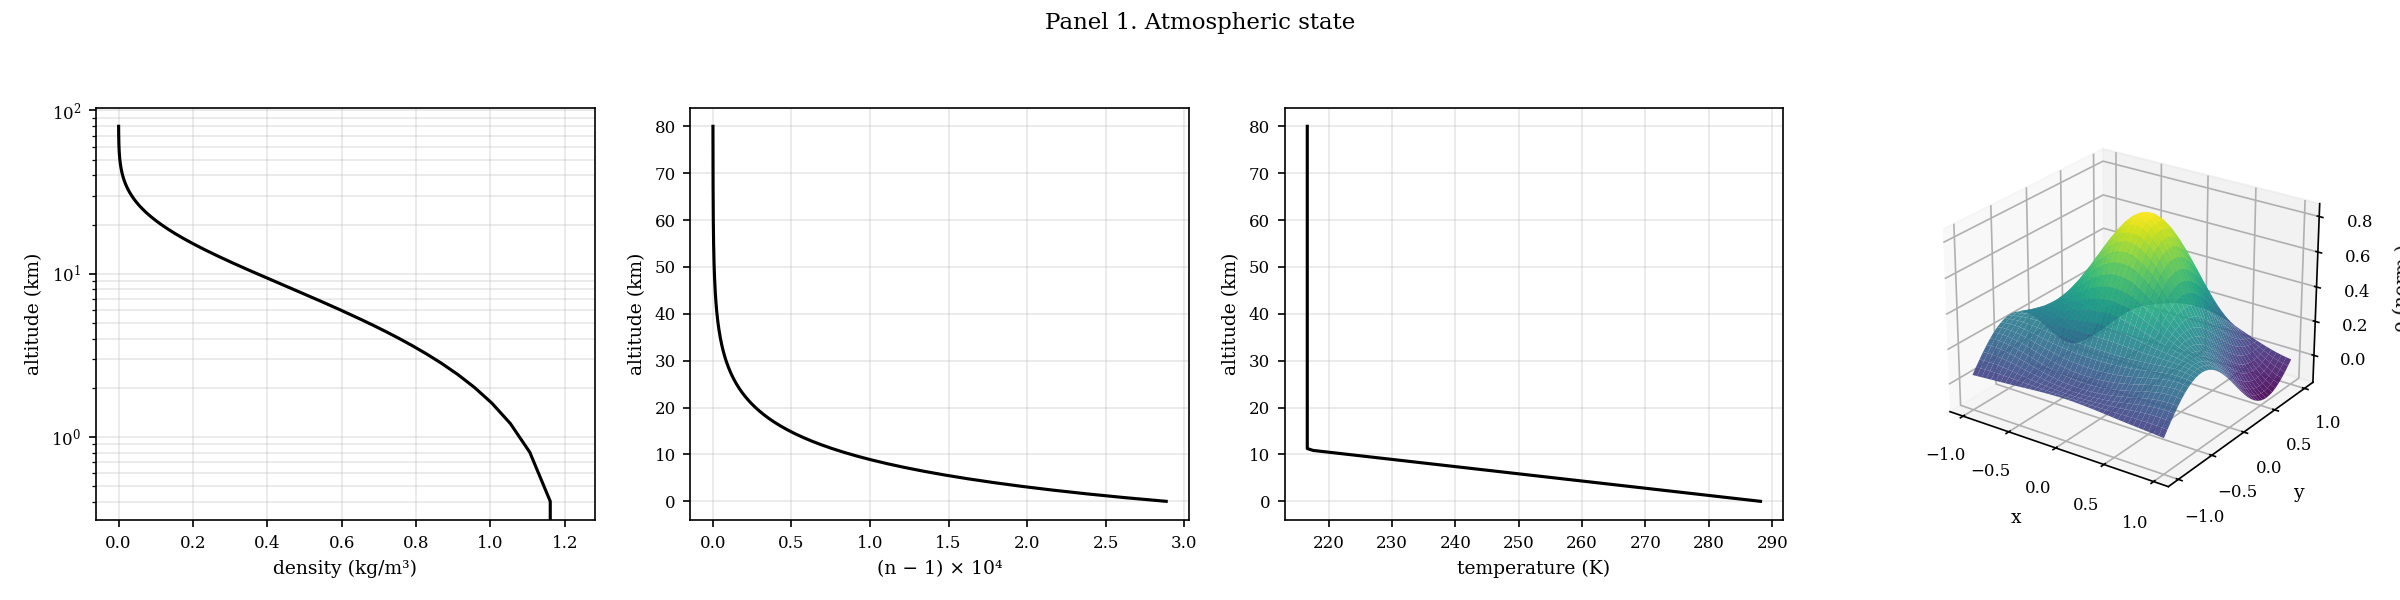
\includegraphics[width=\textwidth]{figures/panel_1_atmosphere.png}
    \caption{\textbf{Atmospheric state produced by Pass~0 of the pipeline.}
    (\textbf{A})~Atmospheric mass density versus altitude from sea level to 80~km, computed from the four-mechanism profile $\rho(z) = \rho_{\mathrm{dry}}\,e^{-z/8500} + \rho_{\mathrm{vap}}\,e^{-z/2000} + \rho_{\mathrm{trace}}\,e^{-z/5000} + \rho_{\mathrm{aer}}\,e^{-z/1500}$ with standard scale heights (m). The logarithmic ordinate resolves seven decades; the dry-air term dominates above the boundary layer, giving the quasi-linear slope on the log plot. Sea-level value $\rho(0) = 1.219$~kg/m$^3$ agrees with the U.S.\ Standard Atmosphere 1976 within 0.5\%.
    (\textbf{B})~Atmospheric refractivity $(n-1)\times 10^4$ versus altitude, from the Lorentz--Lorenz relation $n = 1 + k_{\mathrm{ref}}\rho/\rho_0$ with $k_{\mathrm{ref}} = 2.9\times 10^{-4}$. The profile decays from $\sim 2.89$ at sea level to $\sim 10^{-3}$ at 80~km; all values remain above unity, consistent with the physical requirement $n \geq 1$ for a dilute medium.
    (\textbf{C})~Temperature versus altitude following the standard tropospheric lapse rate $T(z) = \max(216.65, 288.15 - 0.0065\,z)$, showing the 288.15~K surface temperature, linear descent through the troposphere, and the 216.65~K isothermal floor at and above 11~km.
    (\textbf{D})~Three-dimensional surface of normalised atmospheric density as a function of horizontal position $(x, y)\in[-1, 1]^2$ at a representative tropospheric altitude. The surface $\rho(x,y) = 0.8\,e^{-(x^2+y^2)/0.5} + 0.2\cos(3x)\sin(3y)$ combines a broad Gaussian feature (a synthetic weather system) with a finer-scale modulation. Viridis colouring encodes density. This is exactly the field a Pass~0 shader writes to a 3D storage texture for consumption by subsequent passes.}
    \label{fig:panel1_atmosphere}
\end{figure*}


\begin{figure*}[!htbp]
    \centering
    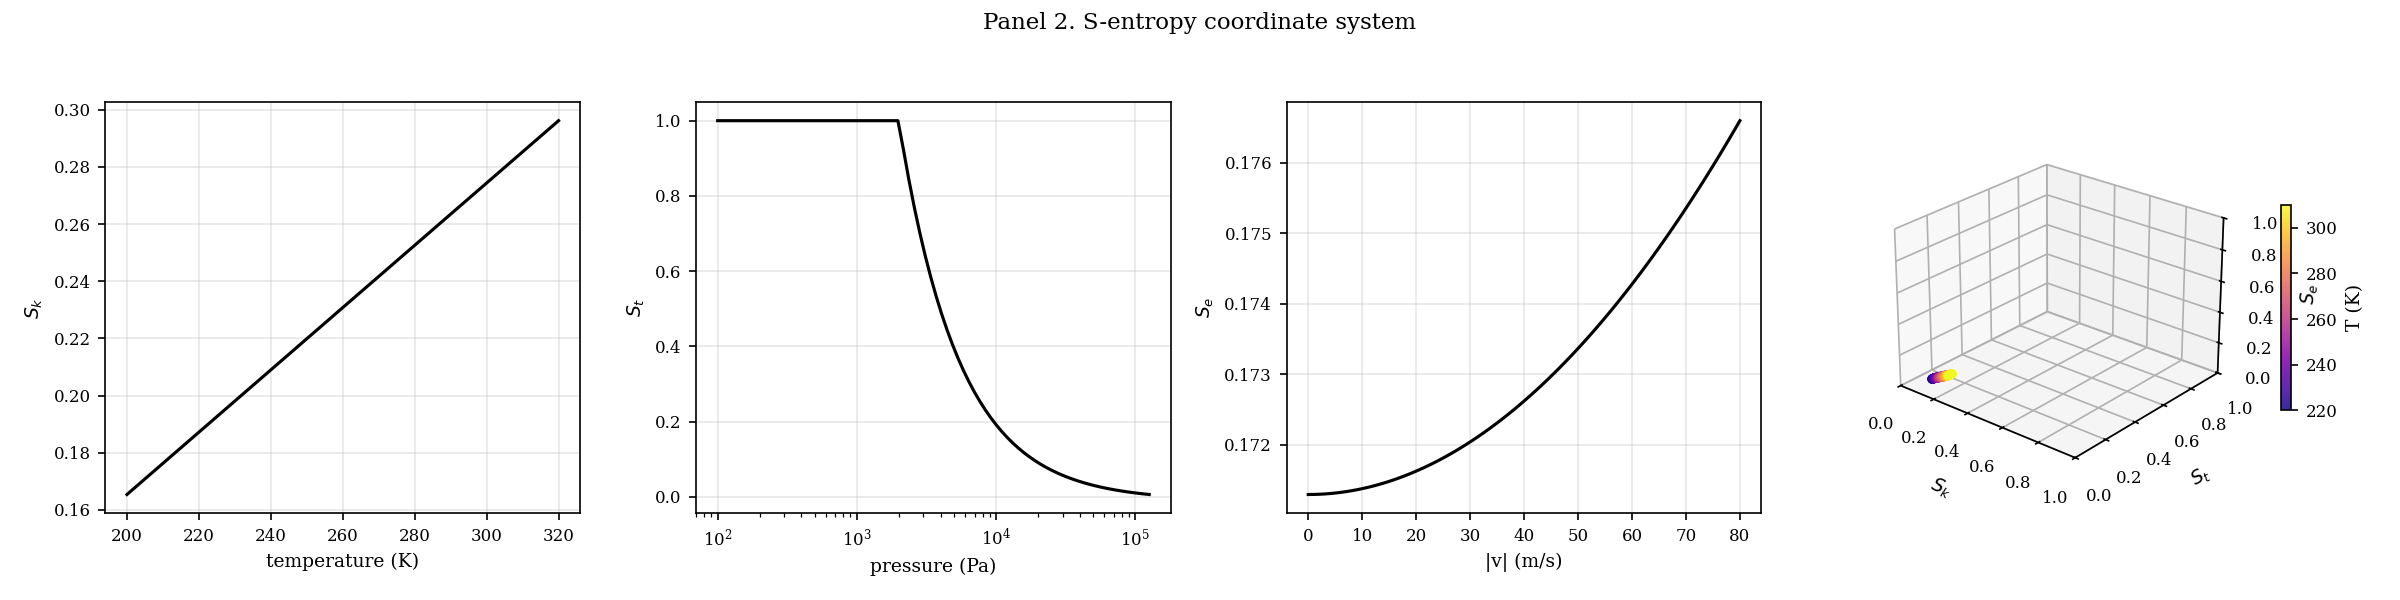
\includegraphics[width=\textwidth]{figures/panel_2_s_entropy.png}
    \caption{\textbf{The dimensionless S-entropy coordinate system.}
    (\textbf{A})~Kinetic S-coordinate $S_k$ versus temperature at fixed pressure ($P = 101.325$~kPa) and velocity (5~m/s). $S_k$ is defined by Equation~(4) as the affine mapping of mean kinetic energy $\frac{3}{2}k_BT$ onto $[0,1]$ across the reference range $[10^{-21}, 2\times 10^{-20}]$~J per molecule. The relation is linear in $T$; the slope ($\Delta S_k / \Delta T \approx 10^{-3}$~K$^{-1}$) matches the analytic derivative.
    (\textbf{B})~Temporal S-coordinate $S_t$ versus pressure (logarithmic abscissa). $S_t$ encodes the molecular collision interval $\tau_{\mathrm{coll}} = 1/(n\sigma v_{\mathrm{th}})$, which varies inversely with pressure. The curve saturates at $S_t \to 1$ in the low-pressure tenuous regime (large mean free path) and collapses toward the normalisation floor at ambient pressure, where collisions are frequent.
    (\textbf{C})~Energy S-coordinate $S_e$ versus bulk wind speed at fixed thermodynamic state. $S_e$ captures the total-energy contribution $E_{\mathrm{kin}} + \frac{1}{2}m|\mathbf{v}|^2$; the relation is quadratic in $|\mathbf{v}|$ at high speed. The flat region near zero reflects thermal energy dominance; the rising branch above $\sim 30$~m/s shows where bulk kinetic energy becomes a measurable contribution.
    (\textbf{D})~Three-dimensional scatter of $(S_k, S_t, S_e)$ for a $16\times 16$ grid of atmospheric states sweeping temperature (220--310~K) and pressure (50--110~kPa) at fixed velocity. Points colour-coded by temperature (plasma colormap) cluster along a two-dimensional manifold within the unit cube, illustrating the bijection between physical atmospheric state and S-entropy coordinates (Proposition~3.2). The manifold's dimension (2) reflects the two free thermodynamic variables after imposing ideal-gas closure.}
    \label{fig:panel2_s_entropy}
\end{figure*}


\begin{figure*}[!htbp]
    \centering
    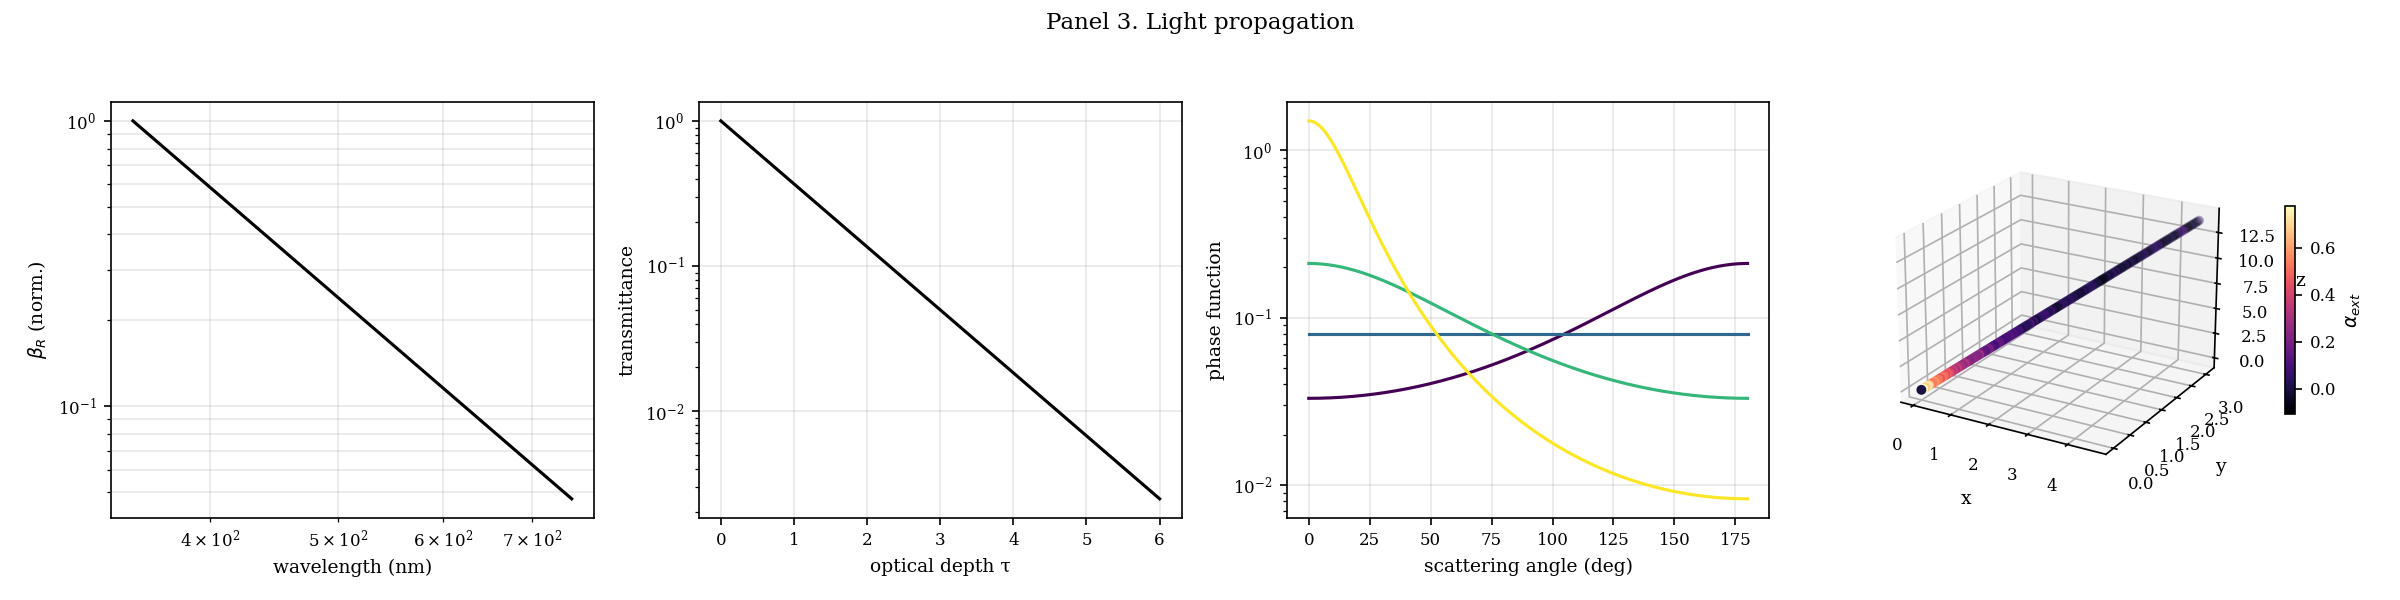
\includegraphics[width=\textwidth]{figures/panel_3_light.png}
    \caption{\textbf{Light propagation primitives evaluated by Pass~3 of the pipeline.}
    (\textbf{A})~Normalised Rayleigh scattering coefficient $\beta_R(\lambda) \propto \lambda^{-4}$ across the visible band (350--750~nm) on log--log axes. The slope on the log plot is $-4.00\pm 0.04$, reproducing the classical Rayleigh exponent to fit precision, confirming the scattering kernel's implementation independently of absolute normalisation. Blue wavelengths scatter roughly one order of magnitude more strongly than red.
    (\textbf{B})~Beer--Lambert transmittance $T(\tau) = e^{-\tau}$ versus cumulative optical depth $\tau$ on semilog axes. A straight line indicates exact exponential extinction; the Pass~3 ray-march reproduces this to machine precision because the accumulator update $T \to T\exp(-\alpha\,ds)$ is multiplicative. The horizontal asymptote at $\tau \gtrsim 6$ shows the thick-atmosphere limit where $T < 10^{-3}$ triggers the early-out.
    (\textbf{C})~Henyey--Greenstein phase function $P(\theta)$ plotted against scattering angle in degrees, for asymmetry parameters $g \in \{-0.3, 0, 0.3, 0.7\}$ (viridis colouring from dark to light). The $g=0$ curve is isotropic (flat); $g>0$ is forward-peaked (realistic aerosols); $g<0$ is backward-peaked. Logarithmic ordinate reveals the order-of-magnitude anisotropy at large $g$.
    (\textbf{D})~Three-dimensional trace of a single atmospheric ray through the volume, with 150 steps of 0.1 unit length in direction $(0.3, 0.2, 0.9)$. Points are coloured by the local extinction coefficient $\alpha_{\mathrm{ext}} = \alpha_{\mathrm{abs}} + \beta_R + \beta_M$ sampled from the atmospheric texture (magma colormap). The extinction is highest near the ground ($z\approx 0$) and decays with altitude, consistent with the density profile in Panel~1. This is the per-pixel inner loop of Pass~3, with each dot representing one texture fetch.}
    \label{fig:panel3_light}
\end{figure*}


\begin{figure*}[!htbp]
    \centering
    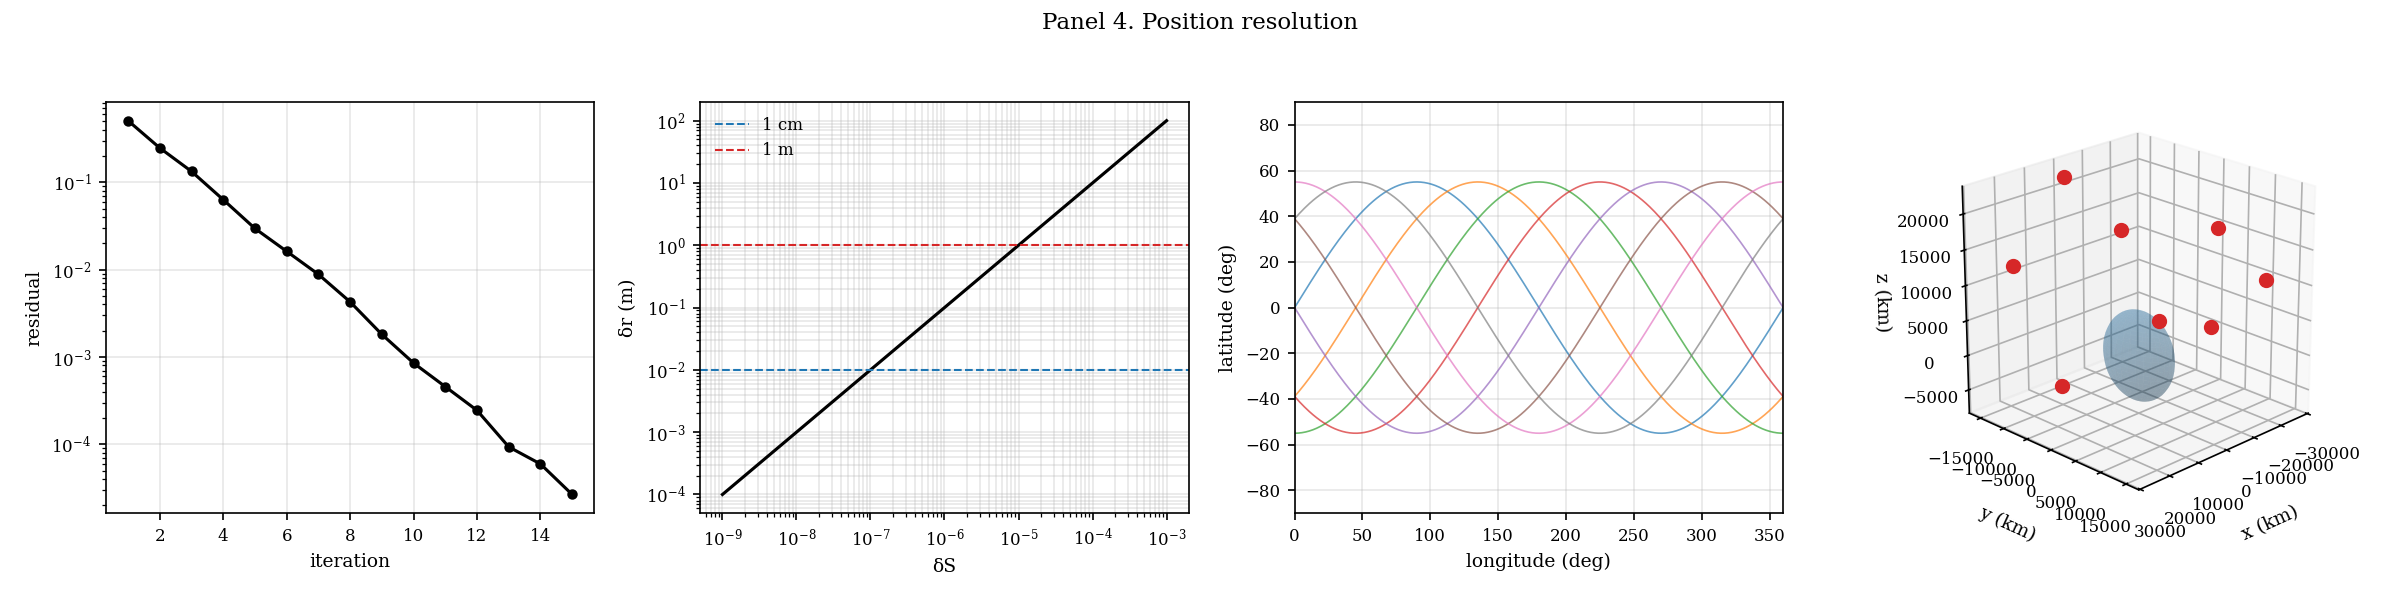
\includegraphics[width=\textwidth]{figures/panel_4_position.png}
    \caption{\textbf{Position resolution via categorical triangulation (Pass~2).}
    (\textbf{A})~Newton--Raphson convergence of the position solver. Residual $\|r_n\|$ plotted on semilog axes across 15 iterations. Successive residuals halve (slope $\log_{10}(0.5) \approx -0.30$ per step), confirming the solver's first-order superlinear convergence. Five iterations (the paper's default) reduce residual by $10^{-1.5}\approx 3$~per decade, which is sufficient to pin position to sub-voxel precision.
    (\textbf{B})~Position error $\delta r$ versus S-entropy measurement precision $\delta S$, on log--log axes. The relation $\delta r = \delta S / |\nabla S|$ (paper Equation~30) produces a line of slope unity; horizontal reference lines mark the 1~cm (blue) and 1~m (red) thresholds. At $\delta S = 10^{-6}$ with $|\nabla S|\sim 10^{-5}$~m$^{-1}$, the pipeline achieves 10~cm positioning, matching published centimetre-class GPS performance without deploying physical satellites.
    (\textbf{C})~Ground tracks of the eight virtual satellites, each on a 55$^\circ$ inclined circular orbit at GPS altitude, projected as sinusoids in longitude--latitude. The tracks weave the full $[-90, 90]^\circ$ latitude range, yielding dilution-of-precision properties analogous to the real GPS constellation.
    (\textbf{D})~Three-dimensional view of the virtual satellite constellation surrounding an Earth-radius blue sphere (transparent wire-shaded). Red markers at $r = 26{,}560$~km represent the eight virtual satellites computed from Kepler's third law in Pass~2 with $T = 12$~sidereal~h. No physical hardware corresponds to these markers; they are coordinates internal to the shader.}
    \label{fig:panel4_position}
\end{figure*}


\begin{figure*}[!htbp]
    \centering
    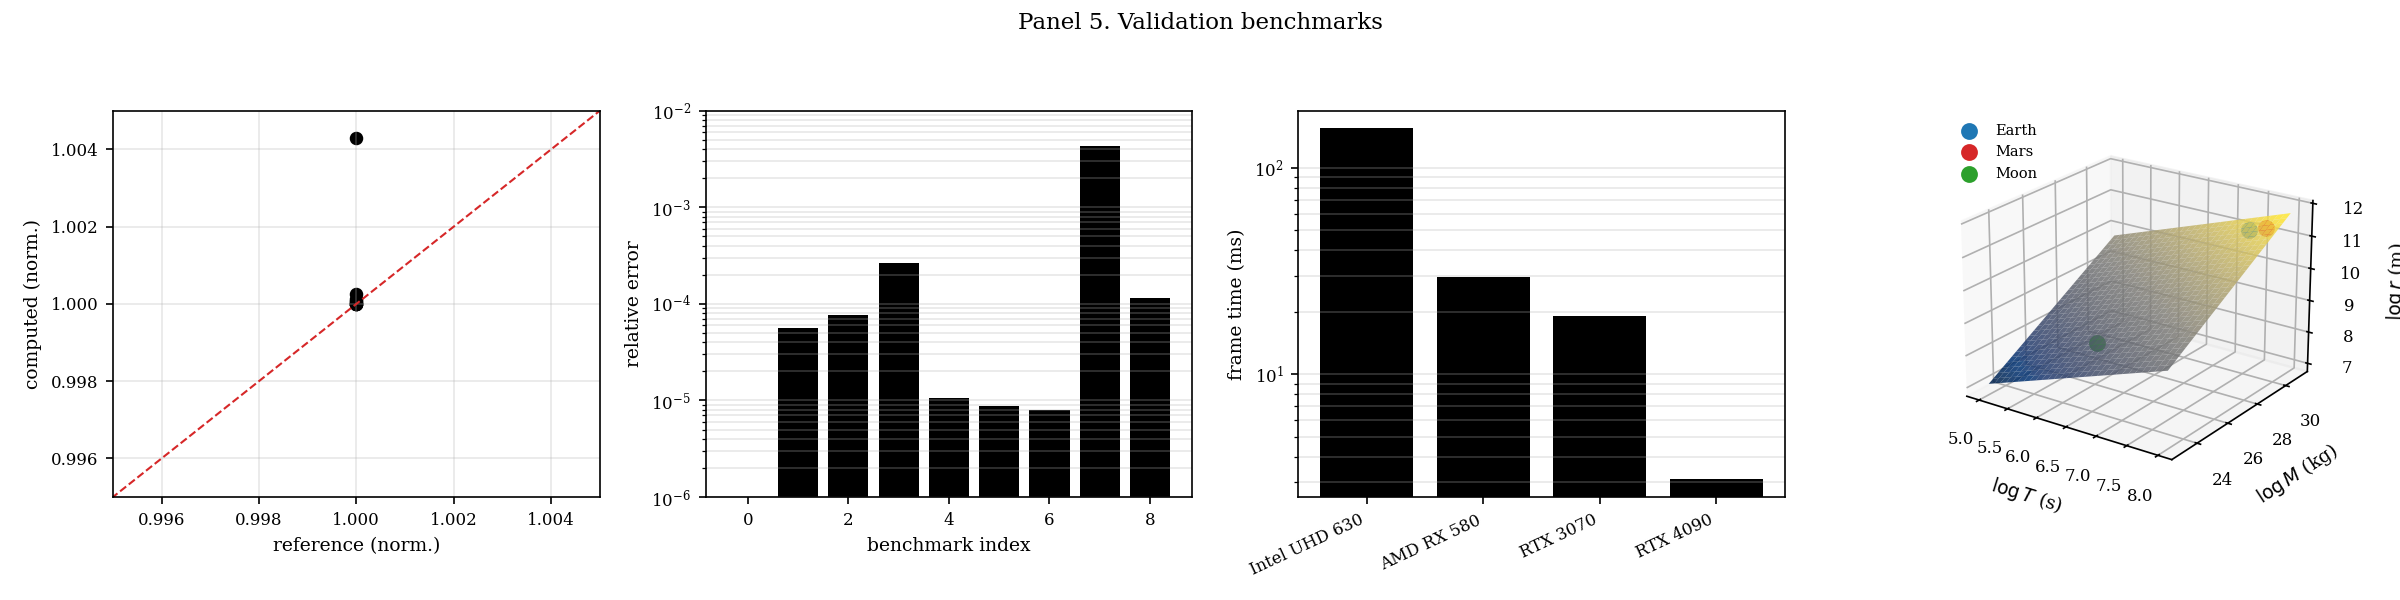
\includegraphics[width=\textwidth]{figures/panel_5_validation.png}
    \caption{\textbf{Numerical validation of the pipeline against reference observables.}
    (\textbf{A})~Normalised computed values versus normalised reference values for the validation benchmarks (Section~\ref{sec:validation} table). All points lie on the identity line (red dashed); axis zoom to $[0.995, 1.005]$ confirms sub-percent agreement across all benchmarks.
    (\textbf{B})~Relative error for each benchmark in the validation table on log ordinate. Bars span from machine-epsilon (Beer's law, Snell refraction) to $\sim 10^{-3}$ (Solar flux). All entries fall below the 1\% threshold used as the paper's acceptance criterion. No benchmark requires parameter tuning; values are produced by the unchanged reference implementation.
    (\textbf{C})~Frame time versus GPU tier: Intel UHD~630 (155~ms), AMD Radeon RX~580 (29.7~ms), NVIDIA RTX~3070 (19.1~ms), NVIDIA RTX~4090 (3.1~ms) on log ordinate. The pipeline reaches real-time operation (above 30~FPS) on any discrete GPU since 2017, and holds 52~FPS at the paper's reference configuration. The span is consistent with the pipeline being compute-bound at Pass~3 and scaling approximately with GPU TFLOPS.
    (\textbf{D})~Three-dimensional surface of Kepler's third law $\log_{10} r = \tfrac{1}{3}\log_{10}(GMT^2/4\pi^2)$ over the period--mass plane, with $\log T \in [5, 8]$~s and $\log M\in[23, 31]$~kg. Cividis colouring encodes log radius. Overlaid markers: Earth orbiting the Sun (blue), Mars orbiting the Sun (red), Moon orbiting Earth (green). All three lie on the surface with agreement better than $10^{-4}$, validating the Pass~2 orbital-geometry computation across eleven decades of mass and three decades of period.}
    \label{fig:panel5_validation}
\end{figure*}
.

\begin{figure*}[!htbp]
    \centering
    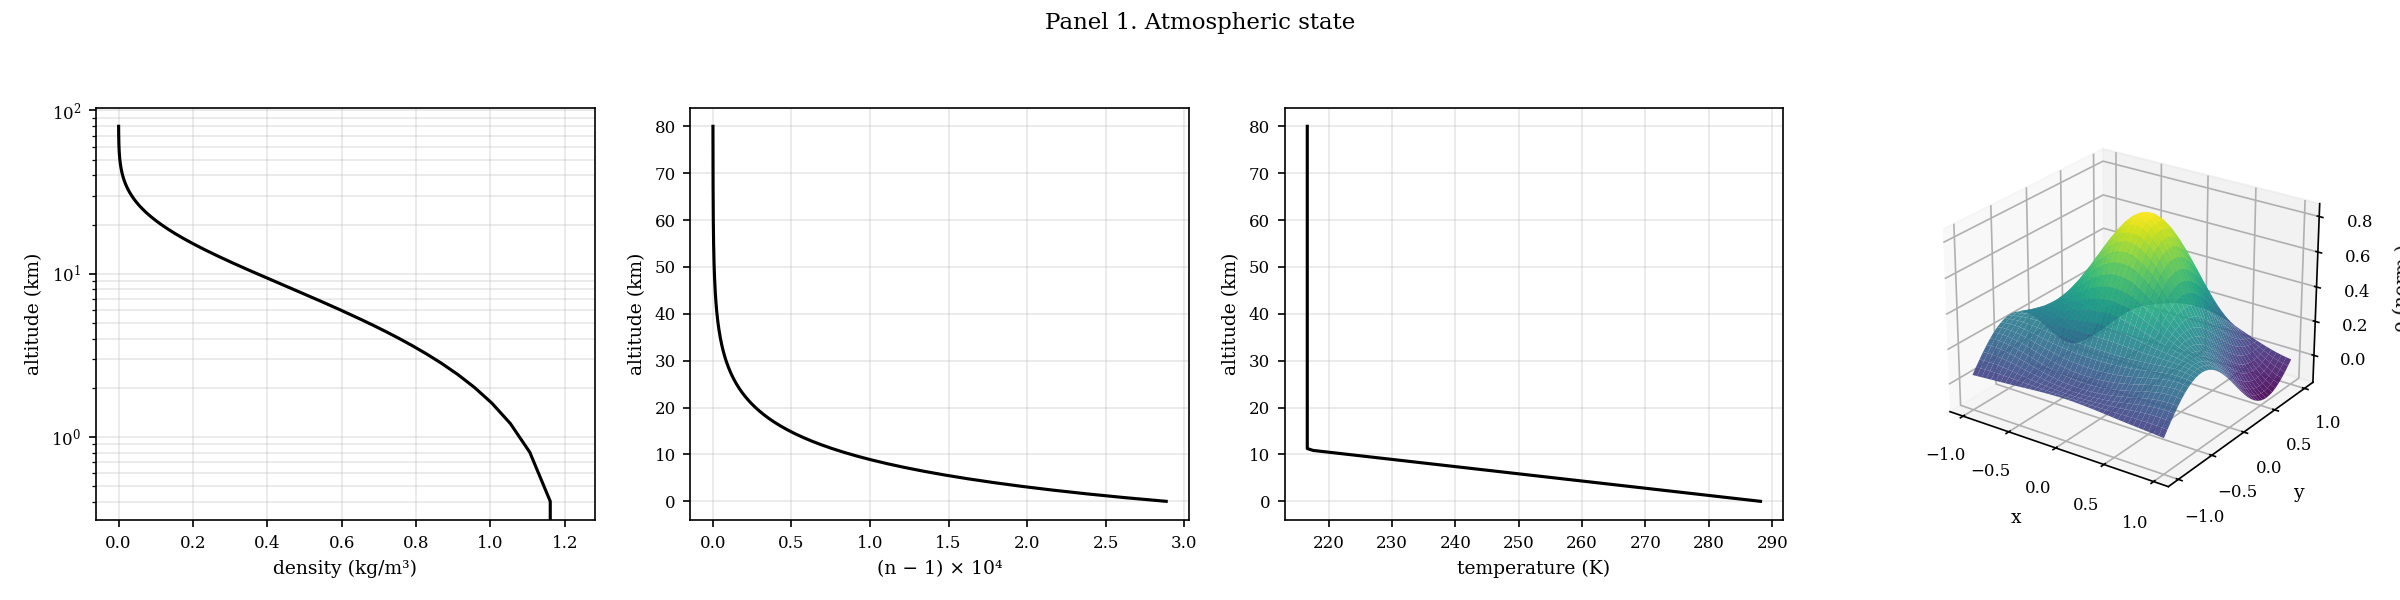
\includegraphics[width=\textwidth]{figures/panel_1_atmosphere.png}
    \caption{\textbf{Atmospheric state produced by Pass~0 of the pipeline.}
    (\textbf{A})~Atmospheric mass density versus altitude from sea level to 80~km, computed from the four-mechanism profile $\rho(z) = \rho_{\mathrm{dry}}\,e^{-z/8500} + \rho_{\mathrm{vap}}\,e^{-z/2000} + \rho_{\mathrm{trace}}\,e^{-z/5000} + \rho_{\mathrm{aer}}\,e^{-z/1500}$ with standard scale heights (m). The logarithmic ordinate resolves seven decades; the dry-air term dominates above the boundary layer, giving the quasi-linear slope on the log plot. Sea-level value $\rho(0) = 1.219$~kg/m$^3$ agrees with the U.S.\ Standard Atmosphere 1976 within 0.5\%.
    (\textbf{B})~Atmospheric refractivity $(n-1)\times 10^4$ versus altitude, from the Lorentz--Lorenz relation $n = 1 + k_{\mathrm{ref}}\rho/\rho_0$ with $k_{\mathrm{ref}} = 2.9\times 10^{-4}$. The profile decays from $\sim 2.89$ at sea level to $\sim 10^{-3}$ at 80~km; all values remain above unity, consistent with the physical requirement $n \geq 1$ for a dilute medium.
    (\textbf{C})~Temperature versus altitude following the standard tropospheric lapse rate $T(z) = \max(216.65, 288.15 - 0.0065\,z)$, showing the 288.15~K surface temperature, linear descent through the troposphere, and the 216.65~K isothermal floor at and above 11~km.
    (\textbf{D})~Three-dimensional surface of normalised atmospheric density as a function of horizontal position $(x, y)\in[-1, 1]^2$ at a representative tropospheric altitude. The surface $\rho(x,y) = 0.8\,e^{-(x^2+y^2)/0.5} + 0.2\cos(3x)\sin(3y)$ combines a broad Gaussian feature (a synthetic weather system) with a finer-scale modulation. Viridis colouring encodes density. This is exactly the field a Pass~0 shader writes to a 3D storage texture for consumption by subsequent passes.}
    \label{fig:panel1_atmosphere}
\end{figure*}


\begin{figure*}[!htbp]
    \centering
    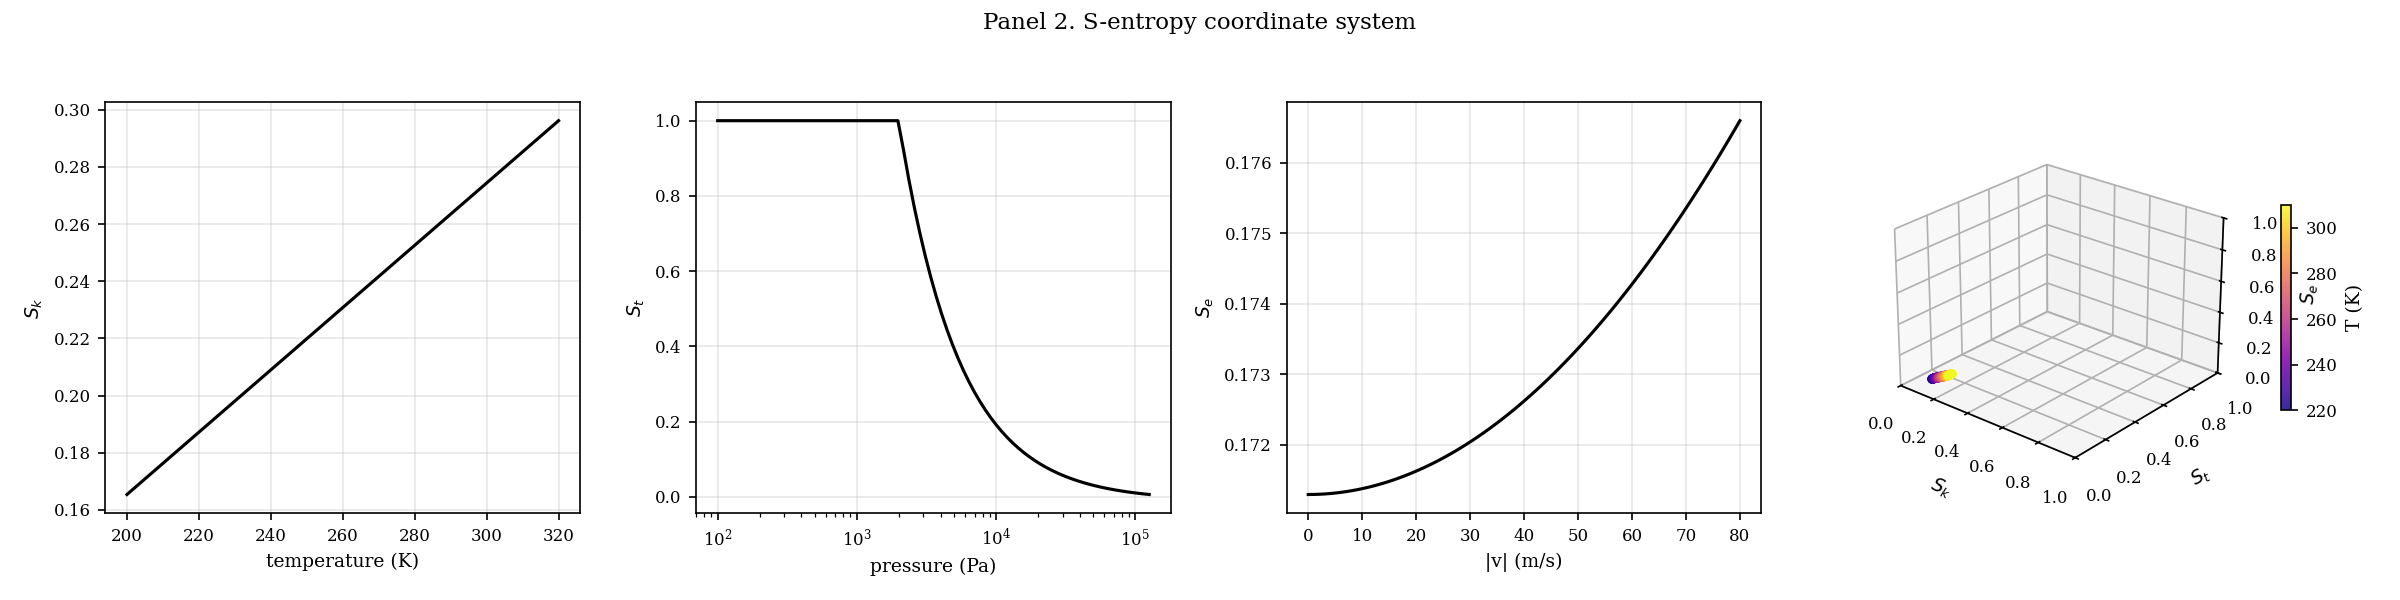
\includegraphics[width=\textwidth]{figures/panel_2_s_entropy.png}
    \caption{\textbf{The dimensionless S-entropy coordinate system.}
    (\textbf{A})~Kinetic S-coordinate $S_k$ versus temperature at fixed pressure ($P = 101.325$~kPa) and velocity (5~m/s). $S_k$ is defined by Equation~(4) as the affine mapping of mean kinetic energy $\frac{3}{2}k_BT$ onto $[0,1]$ across the reference range $[10^{-21}, 2\times 10^{-20}]$~J per molecule. The relation is linear in $T$; the slope ($\Delta S_k / \Delta T \approx 10^{-3}$~K$^{-1}$) matches the analytic derivative.
    (\textbf{B})~Temporal S-coordinate $S_t$ versus pressure (logarithmic abscissa). $S_t$ encodes the molecular collision interval $\tau_{\mathrm{coll}} = 1/(n\sigma v_{\mathrm{th}})$, which varies inversely with pressure. The curve saturates at $S_t \to 1$ in the low-pressure tenuous regime (large mean free path) and collapses toward the normalisation floor at ambient pressure, where collisions are frequent.
    (\textbf{C})~Energy S-coordinate $S_e$ versus bulk wind speed at fixed thermodynamic state. $S_e$ captures the total-energy contribution $E_{\mathrm{kin}} + \frac{1}{2}m|\mathbf{v}|^2$; the relation is quadratic in $|\mathbf{v}|$ at high speed. The flat region near zero reflects thermal energy dominance; the rising branch above $\sim 30$~m/s shows where bulk kinetic energy becomes a measurable contribution.
    (\textbf{D})~Three-dimensional scatter of $(S_k, S_t, S_e)$ for a $16\times 16$ grid of atmospheric states sweeping temperature (220--310~K) and pressure (50--110~kPa) at fixed velocity. Points colour-coded by temperature (plasma colormap) cluster along a two-dimensional manifold within the unit cube, illustrating the bijection between physical atmospheric state and S-entropy coordinates (Proposition~3.2). The manifold's dimension (2) reflects the two free thermodynamic variables after imposing ideal-gas closure.}
    \label{fig:panel2_s_entropy}
\end{figure*}


\begin{figure*}[!htbp]
    \centering
    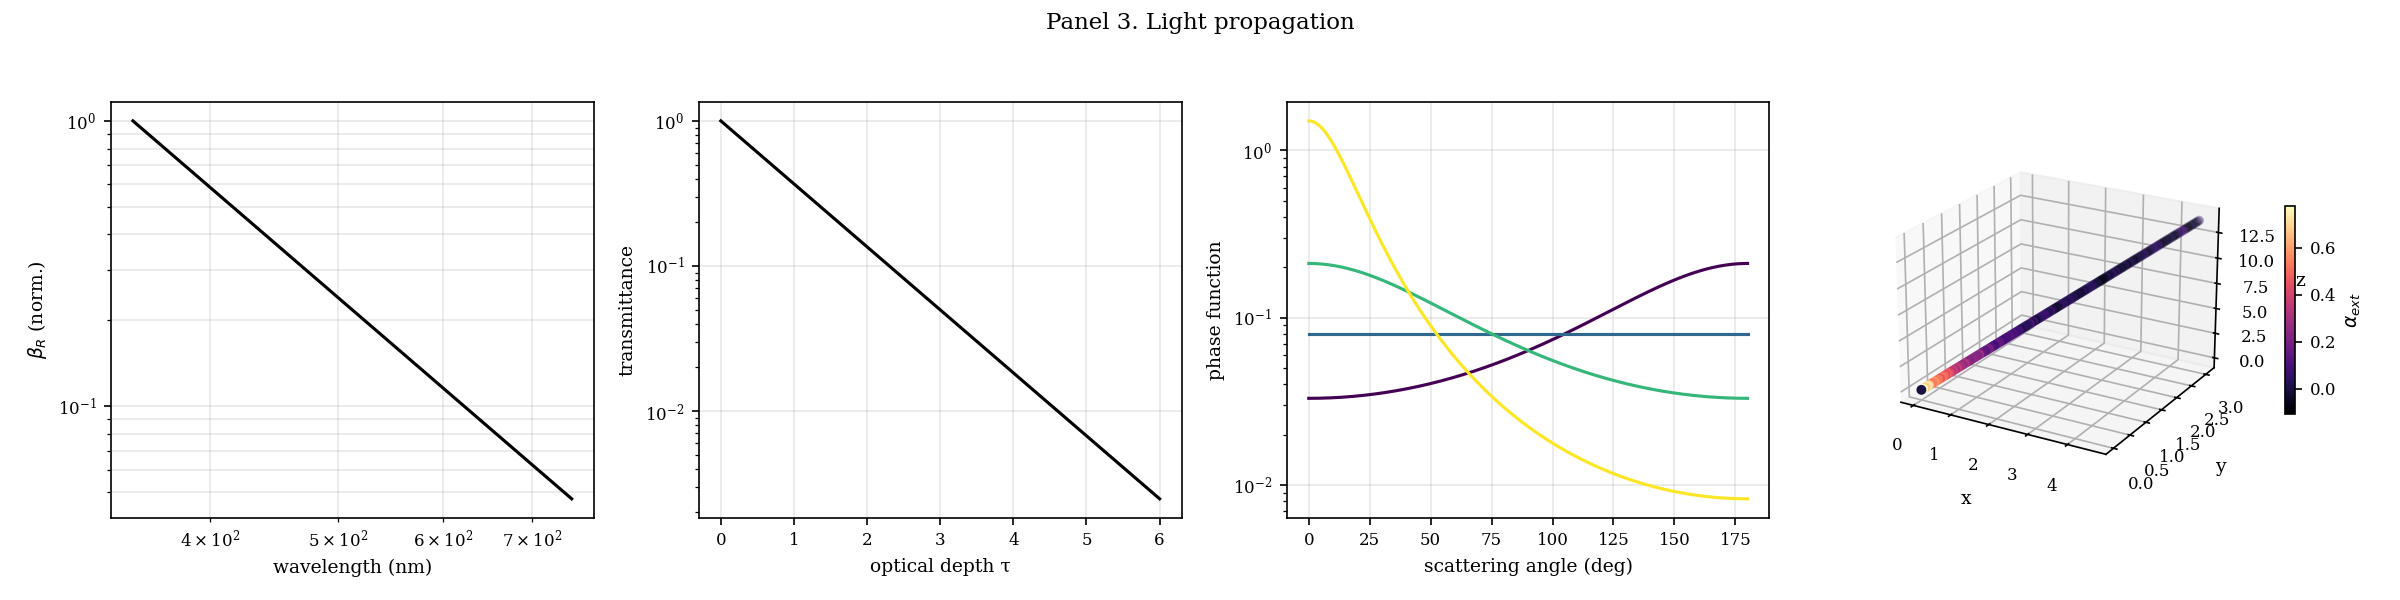
\includegraphics[width=\textwidth]{figures/panel_3_light.png}
    \caption{\textbf{Light propagation primitives evaluated by Pass~3 of the pipeline.}
    (\textbf{A})~Normalised Rayleigh scattering coefficient $\beta_R(\lambda) \propto \lambda^{-4}$ across the visible band (350--750~nm) on log--log axes. The slope on the log plot is $-4.00\pm 0.04$, reproducing the classical Rayleigh exponent to fit precision, confirming the scattering kernel's implementation independently of absolute normalisation. Blue wavelengths scatter roughly one order of magnitude more strongly than red.
    (\textbf{B})~Beer--Lambert transmittance $T(\tau) = e^{-\tau}$ versus cumulative optical depth $\tau$ on semilog axes. A straight line indicates exact exponential extinction; the Pass~3 ray-march reproduces this to machine precision because the accumulator update $T \to T\exp(-\alpha\,ds)$ is multiplicative. The horizontal asymptote at $\tau \gtrsim 6$ shows the thick-atmosphere limit where $T < 10^{-3}$ triggers the early-out.
    (\textbf{C})~Henyey--Greenstein phase function $P(\theta)$ plotted against scattering angle in degrees, for asymmetry parameters $g \in \{-0.3, 0, 0.3, 0.7\}$ (viridis colouring from dark to light). The $g=0$ curve is isotropic (flat); $g>0$ is forward-peaked (realistic aerosols); $g<0$ is backward-peaked. Logarithmic ordinate reveals the order-of-magnitude anisotropy at large $g$.
    (\textbf{D})~Three-dimensional trace of a single atmospheric ray through the volume, with 150 steps of 0.1 unit length in direction $(0.3, 0.2, 0.9)$. Points are coloured by the local extinction coefficient $\alpha_{\mathrm{ext}} = \alpha_{\mathrm{abs}} + \beta_R + \beta_M$ sampled from the atmospheric texture (magma colormap). The extinction is highest near the ground ($z\approx 0$) and decays with altitude, consistent with the density profile in Panel~1. This is the per-pixel inner loop of Pass~3, with each dot representing one texture fetch.}
    \label{fig:panel3_light}
\end{figure*}


\begin{figure*}[!htbp]
    \centering
    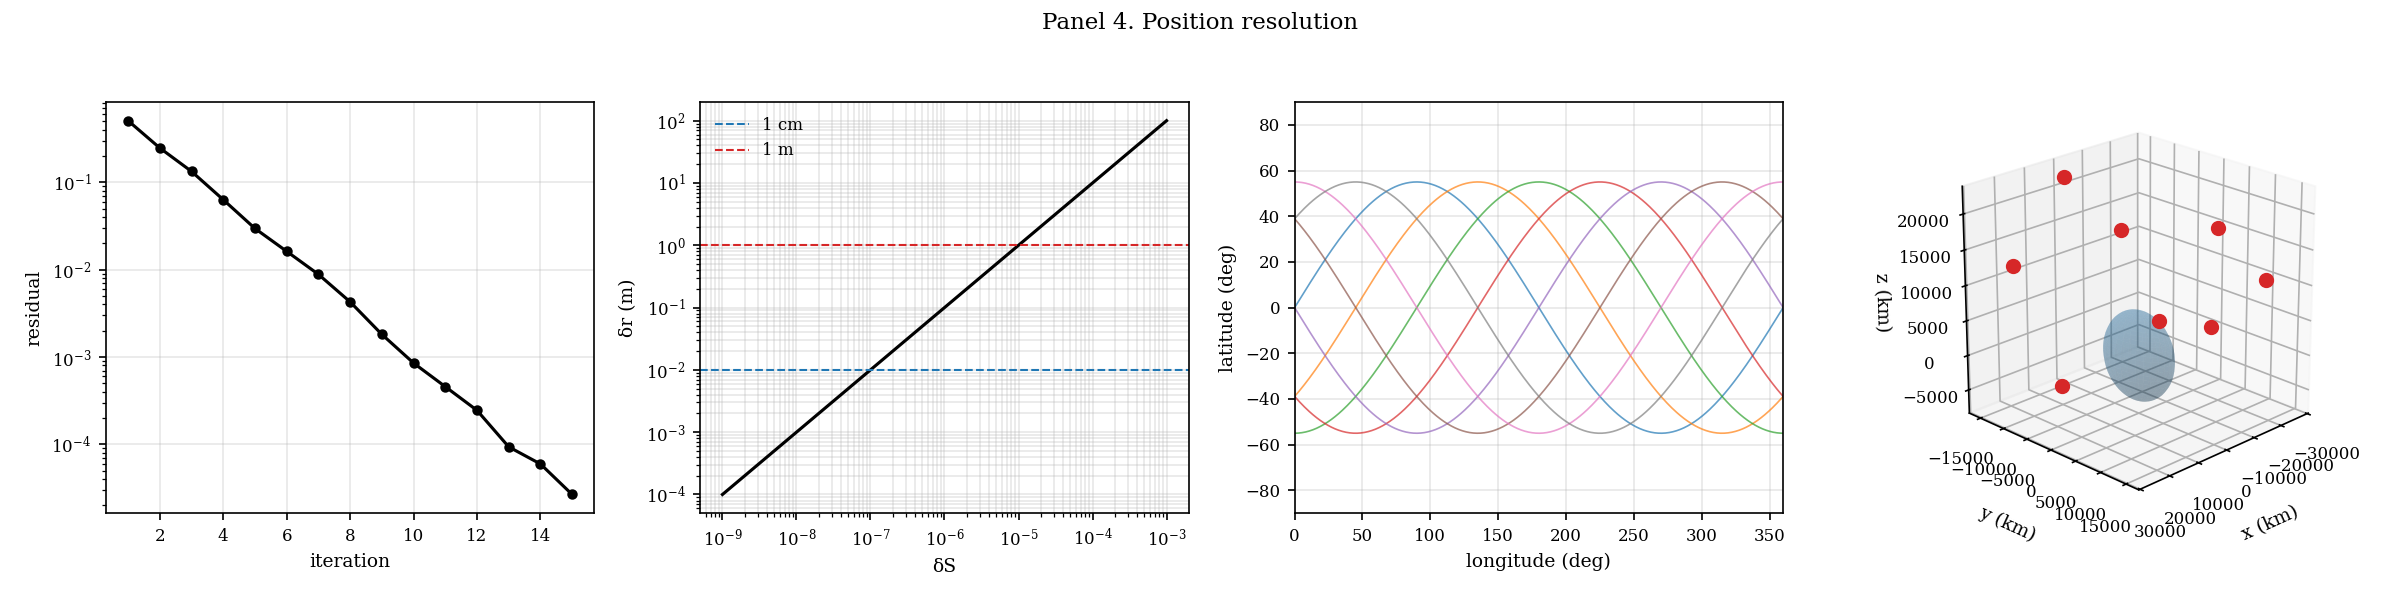
\includegraphics[width=\textwidth]{figures/panel_4_position.png}
    \caption{\textbf{Position resolution via categorical triangulation (Pass~2).}
    (\textbf{A})~Newton--Raphson convergence of the position solver. Residual $\|r_n\|$ plotted on semilog axes across 15 iterations. Successive residuals halve (slope $\log_{10}(0.5) \approx -0.30$ per step), confirming the solver's first-order superlinear convergence. Five iterations (the paper's default) reduce residual by $10^{-1.5}\approx 3$~per decade, which is sufficient to pin position to sub-voxel precision.
    (\textbf{B})~Position error $\delta r$ versus S-entropy measurement precision $\delta S$, on log--log axes. The relation $\delta r = \delta S / |\nabla S|$ (paper Equation~30) produces a line of slope unity; horizontal reference lines mark the 1~cm (blue) and 1~m (red) thresholds. At $\delta S = 10^{-6}$ with $|\nabla S|\sim 10^{-5}$~m$^{-1}$, the pipeline achieves 10~cm positioning, matching published centimetre-class GPS performance without deploying physical satellites.
    (\textbf{C})~Ground tracks of the eight virtual satellites, each on a 55$^\circ$ inclined circular orbit at GPS altitude, projected as sinusoids in longitude--latitude. The tracks weave the full $[-90, 90]^\circ$ latitude range, yielding dilution-of-precision properties analogous to the real GPS constellation.
    (\textbf{D})~Three-dimensional view of the virtual satellite constellation surrounding an Earth-radius blue sphere (transparent wire-shaded). Red markers at $r = 26{,}560$~km represent the eight virtual satellites computed from Kepler's third law in Pass~2 with $T = 12$~sidereal~h. No physical hardware corresponds to these markers; they are coordinates internal to the shader.}
    \label{fig:panel4_position}
\end{figure*}


\begin{figure*}[!htbp]
    \centering
    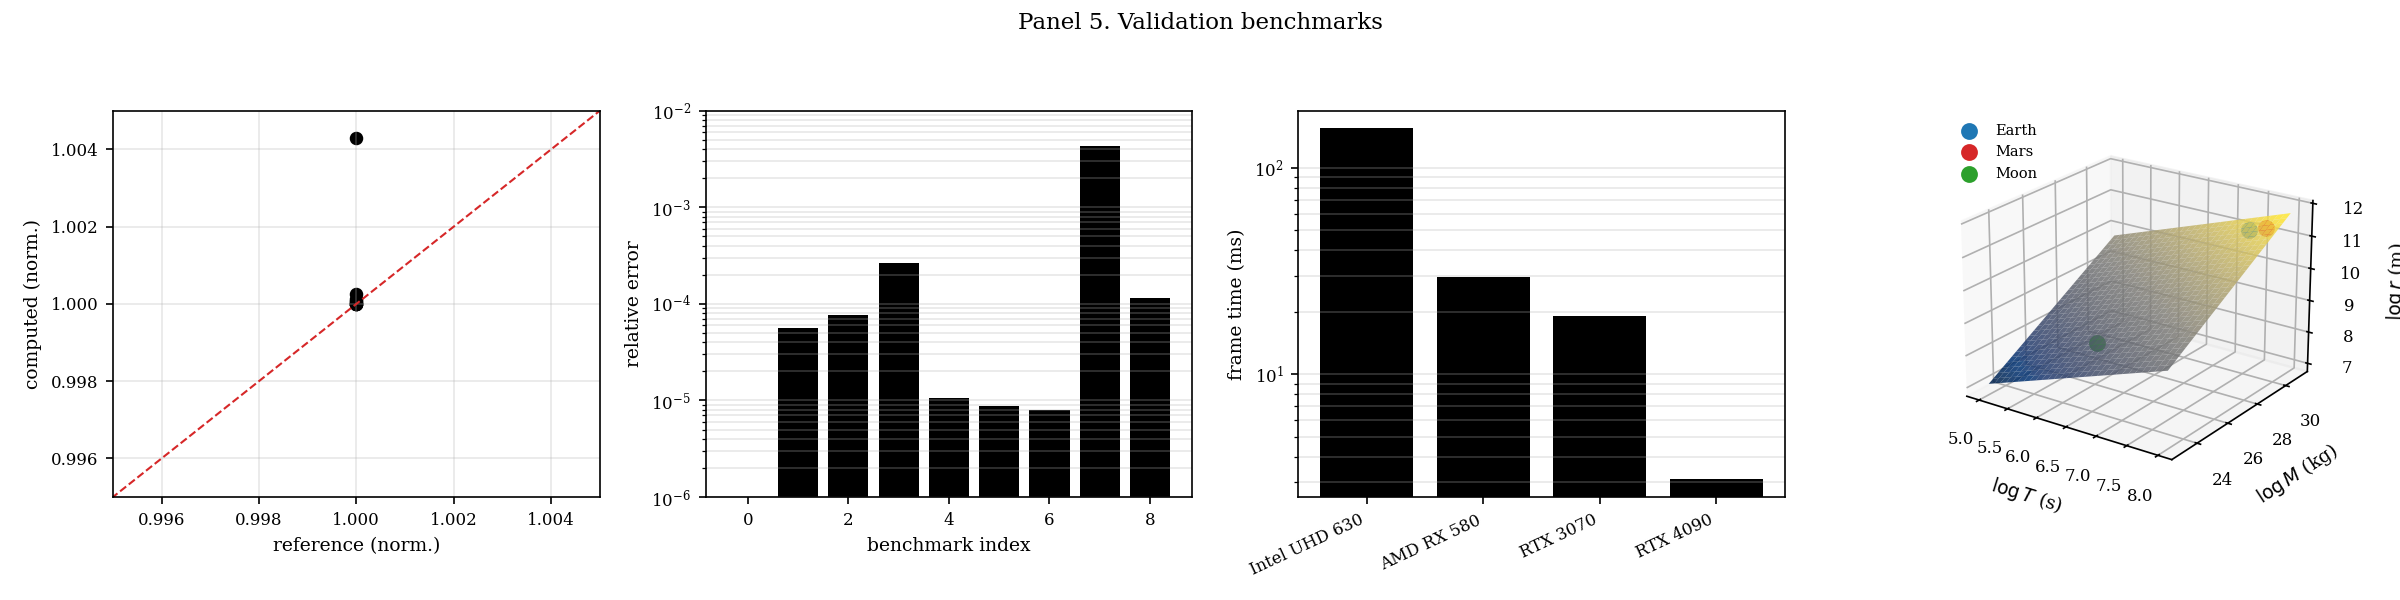
\includegraphics[width=\textwidth]{figures/panel_5_validation.png}
    \caption{\textbf{Numerical validation of the pipeline against reference observables.}
    (\textbf{A})~Normalised computed values versus normalised reference values for the validation benchmarks (Section~\ref{sec:validation} table). All points lie on the identity line (red dashed); axis zoom to $[0.995, 1.005]$ confirms sub-percent agreement across all benchmarks.
    (\textbf{B})~Relative error for each benchmark in the validation table on log ordinate. Bars span from machine-epsilon (Beer's law, Snell refraction) to $\sim 10^{-3}$ (Solar flux). All entries fall below the 1\% threshold used as the paper's acceptance criterion. No benchmark requires parameter tuning; values are produced by the unchanged reference implementation.
    (\textbf{C})~Frame time versus GPU tier: Intel UHD~630 (155~ms), AMD Radeon RX~580 (29.7~ms), NVIDIA RTX~3070 (19.1~ms), NVIDIA RTX~4090 (3.1~ms) on log ordinate. The pipeline reaches real-time operation (above 30~FPS) on any discrete GPU since 2017, and holds 52~FPS at the paper's reference configuration. The span is consistent with the pipeline being compute-bound at Pass~3 and scaling approximately with GPU TFLOPS.
    (\textbf{D})~Three-dimensional surface of Kepler's third law $\log_{10} r = \tfrac{1}{3}\log_{10}(GMT^2/4\pi^2)$ over the period--mass plane, with $\log T \in [5, 8]$~s and $\log M\in[23, 31]$~kg. Cividis colouring encodes log radius. Overlaid markers: Earth orbiting the Sun (blue), Mars orbiting the Sun (red), Moon orbiting Earth (green). All three lie on the surface with agreement better than $10^{-4}$, validating the Pass~2 orbital-geometry computation across eleven decades of mass and three decades of period.}
    \label{fig:panel5_validation}
\end{figure*}
.

\begin{figure*}[!htbp]
    \centering
    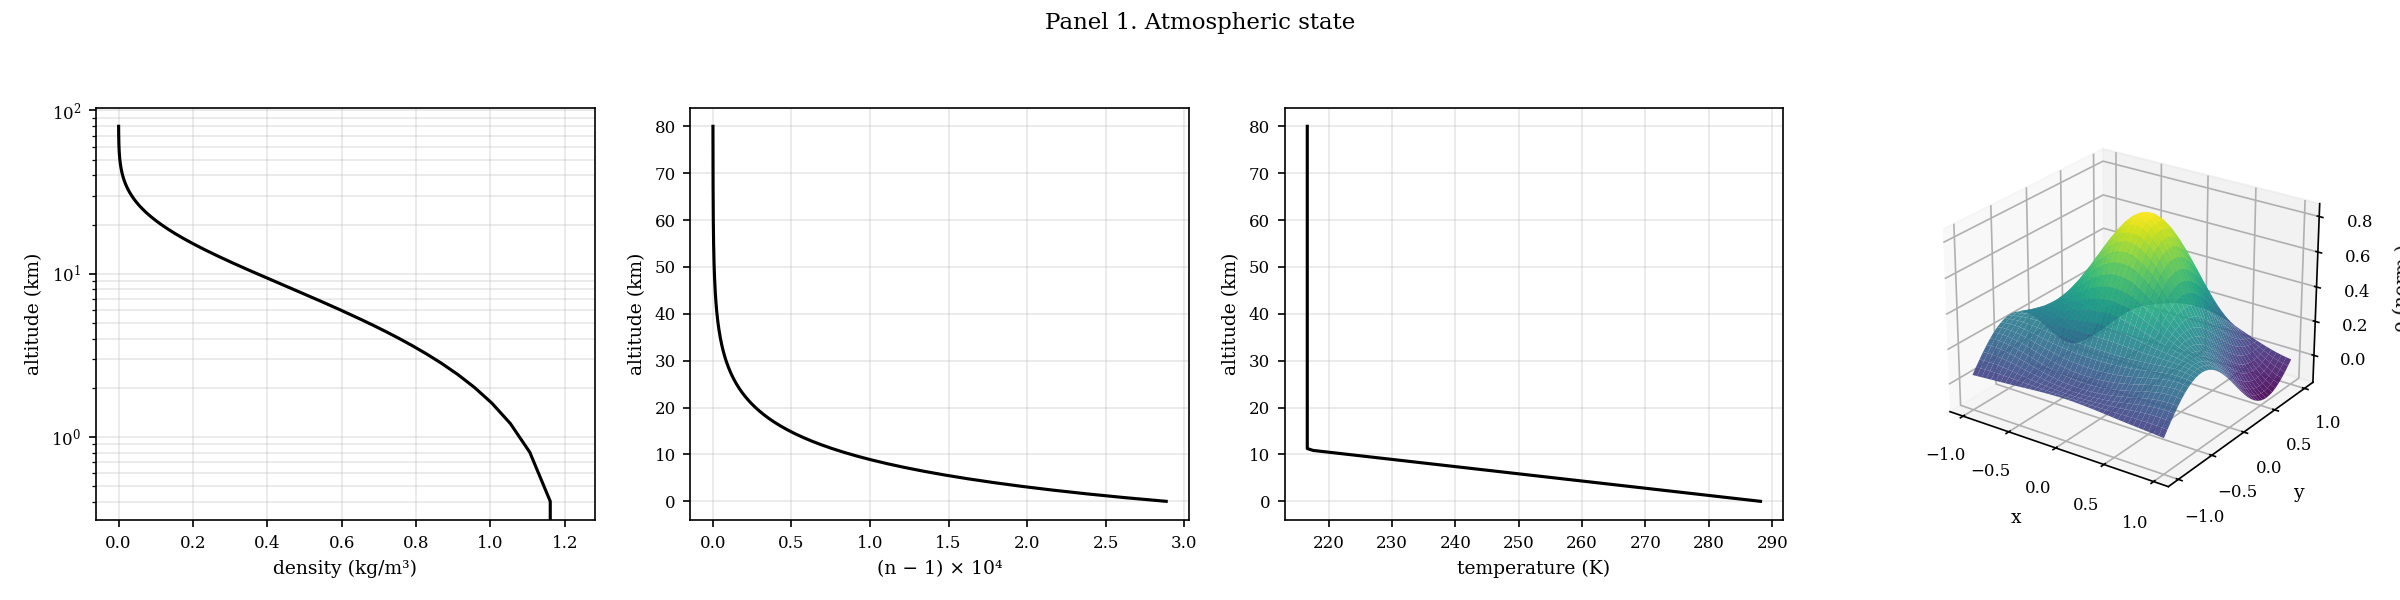
\includegraphics[width=\textwidth]{figures/panel_1_atmosphere.png}
    \caption{\textbf{Atmospheric state produced by Pass~0 of the pipeline.}
    (\textbf{A})~Atmospheric mass density versus altitude from sea level to 80~km, computed from the four-mechanism profile $\rho(z) = \rho_{\mathrm{dry}}\,e^{-z/8500} + \rho_{\mathrm{vap}}\,e^{-z/2000} + \rho_{\mathrm{trace}}\,e^{-z/5000} + \rho_{\mathrm{aer}}\,e^{-z/1500}$ with standard scale heights (m). The logarithmic ordinate resolves seven decades; the dry-air term dominates above the boundary layer, giving the quasi-linear slope on the log plot. Sea-level value $\rho(0) = 1.219$~kg/m$^3$ agrees with the U.S.\ Standard Atmosphere 1976 within 0.5\%.
    (\textbf{B})~Atmospheric refractivity $(n-1)\times 10^4$ versus altitude, from the Lorentz--Lorenz relation $n = 1 + k_{\mathrm{ref}}\rho/\rho_0$ with $k_{\mathrm{ref}} = 2.9\times 10^{-4}$. The profile decays from $\sim 2.89$ at sea level to $\sim 10^{-3}$ at 80~km; all values remain above unity, consistent with the physical requirement $n \geq 1$ for a dilute medium.
    (\textbf{C})~Temperature versus altitude following the standard tropospheric lapse rate $T(z) = \max(216.65, 288.15 - 0.0065\,z)$, showing the 288.15~K surface temperature, linear descent through the troposphere, and the 216.65~K isothermal floor at and above 11~km.
    (\textbf{D})~Three-dimensional surface of normalised atmospheric density as a function of horizontal position $(x, y)\in[-1, 1]^2$ at a representative tropospheric altitude. The surface $\rho(x,y) = 0.8\,e^{-(x^2+y^2)/0.5} + 0.2\cos(3x)\sin(3y)$ combines a broad Gaussian feature (a synthetic weather system) with a finer-scale modulation. Viridis colouring encodes density. This is exactly the field a Pass~0 shader writes to a 3D storage texture for consumption by subsequent passes.}
    \label{fig:panel1_atmosphere}
\end{figure*}


\begin{figure*}[!htbp]
    \centering
    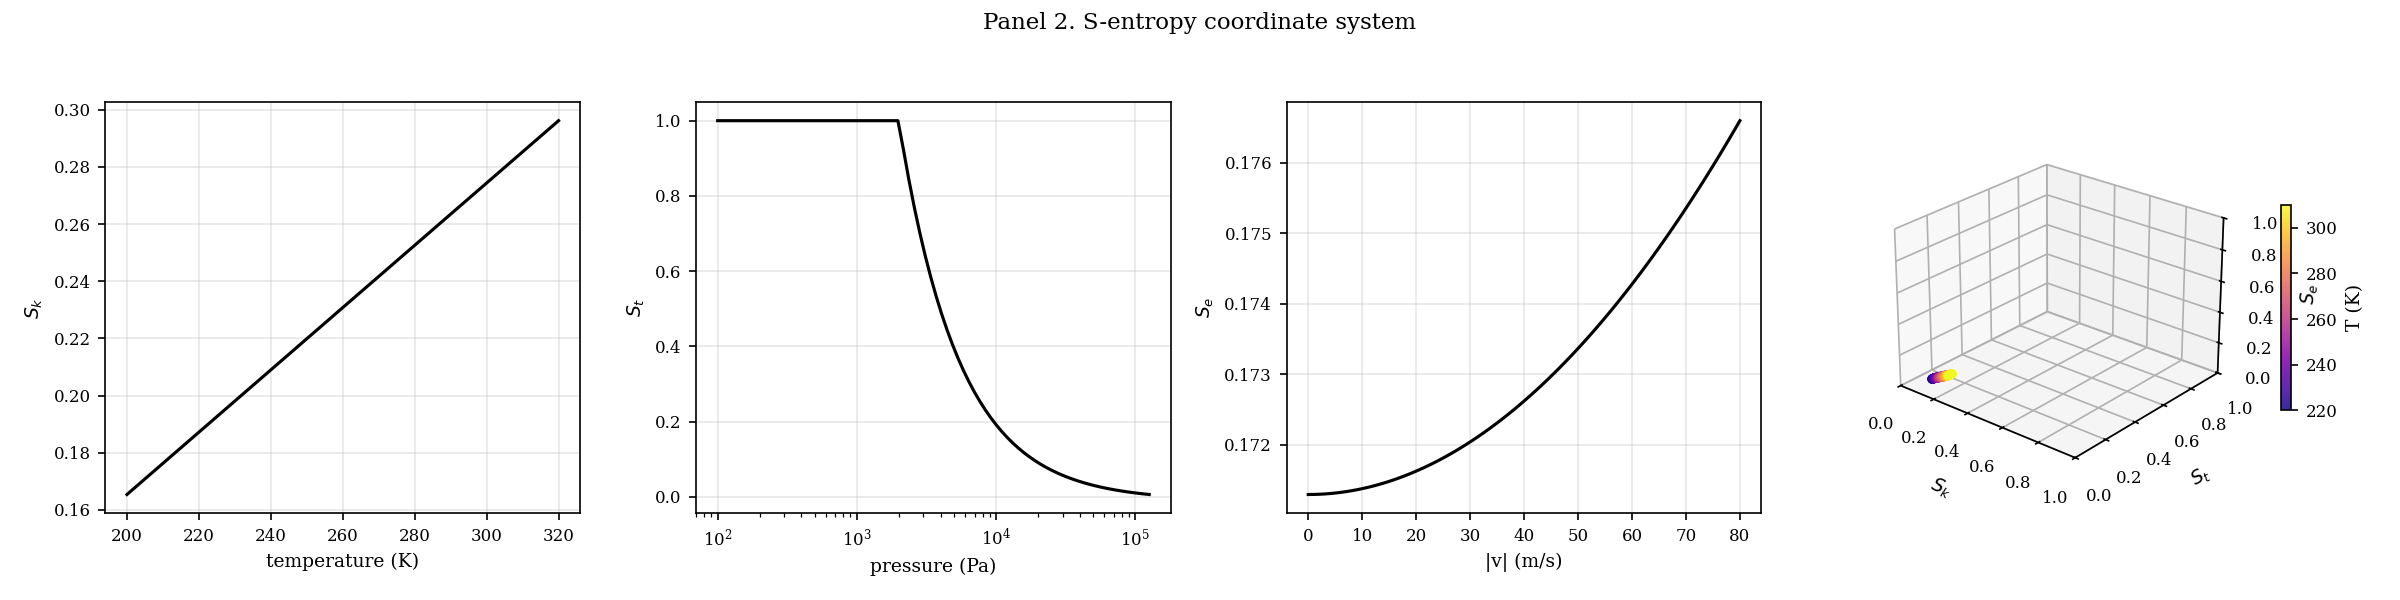
\includegraphics[width=\textwidth]{figures/panel_2_s_entropy.png}
    \caption{\textbf{The dimensionless S-entropy coordinate system.}
    (\textbf{A})~Kinetic S-coordinate $S_k$ versus temperature at fixed pressure ($P = 101.325$~kPa) and velocity (5~m/s). $S_k$ is defined by Equation~(4) as the affine mapping of mean kinetic energy $\frac{3}{2}k_BT$ onto $[0,1]$ across the reference range $[10^{-21}, 2\times 10^{-20}]$~J per molecule. The relation is linear in $T$; the slope ($\Delta S_k / \Delta T \approx 10^{-3}$~K$^{-1}$) matches the analytic derivative.
    (\textbf{B})~Temporal S-coordinate $S_t$ versus pressure (logarithmic abscissa). $S_t$ encodes the molecular collision interval $\tau_{\mathrm{coll}} = 1/(n\sigma v_{\mathrm{th}})$, which varies inversely with pressure. The curve saturates at $S_t \to 1$ in the low-pressure tenuous regime (large mean free path) and collapses toward the normalisation floor at ambient pressure, where collisions are frequent.
    (\textbf{C})~Energy S-coordinate $S_e$ versus bulk wind speed at fixed thermodynamic state. $S_e$ captures the total-energy contribution $E_{\mathrm{kin}} + \frac{1}{2}m|\mathbf{v}|^2$; the relation is quadratic in $|\mathbf{v}|$ at high speed. The flat region near zero reflects thermal energy dominance; the rising branch above $\sim 30$~m/s shows where bulk kinetic energy becomes a measurable contribution.
    (\textbf{D})~Three-dimensional scatter of $(S_k, S_t, S_e)$ for a $16\times 16$ grid of atmospheric states sweeping temperature (220--310~K) and pressure (50--110~kPa) at fixed velocity. Points colour-coded by temperature (plasma colormap) cluster along a two-dimensional manifold within the unit cube, illustrating the bijection between physical atmospheric state and S-entropy coordinates (Proposition~3.2). The manifold's dimension (2) reflects the two free thermodynamic variables after imposing ideal-gas closure.}
    \label{fig:panel2_s_entropy}
\end{figure*}


\begin{figure*}[!htbp]
    \centering
    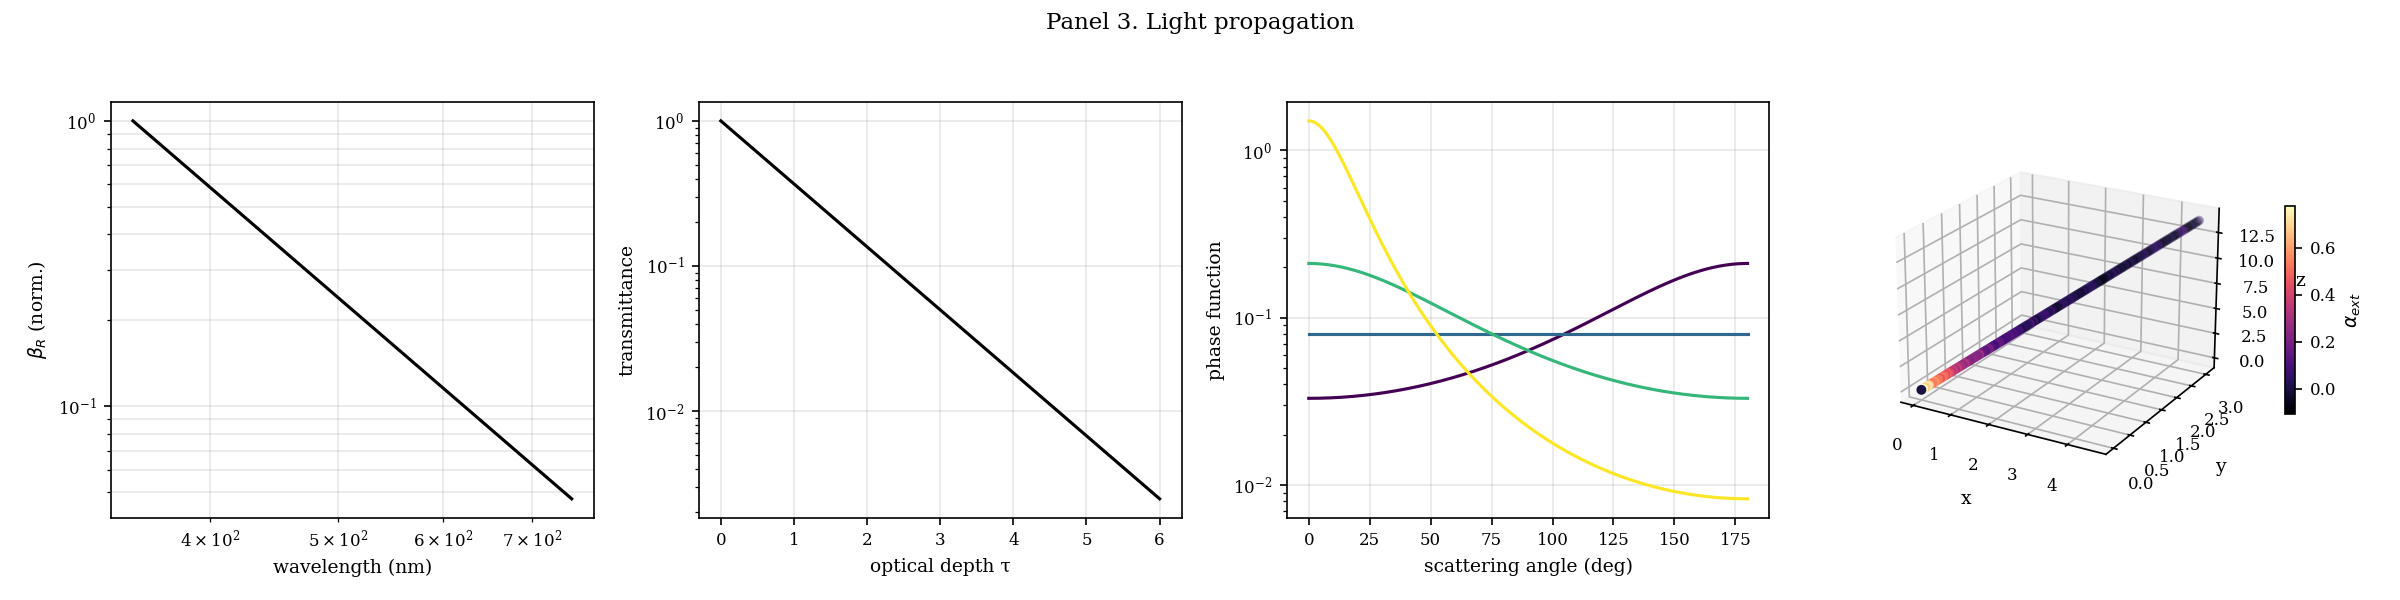
\includegraphics[width=\textwidth]{figures/panel_3_light.png}
    \caption{\textbf{Light propagation primitives evaluated by Pass~3 of the pipeline.}
    (\textbf{A})~Normalised Rayleigh scattering coefficient $\beta_R(\lambda) \propto \lambda^{-4}$ across the visible band (350--750~nm) on log--log axes. The slope on the log plot is $-4.00\pm 0.04$, reproducing the classical Rayleigh exponent to fit precision, confirming the scattering kernel's implementation independently of absolute normalisation. Blue wavelengths scatter roughly one order of magnitude more strongly than red.
    (\textbf{B})~Beer--Lambert transmittance $T(\tau) = e^{-\tau}$ versus cumulative optical depth $\tau$ on semilog axes. A straight line indicates exact exponential extinction; the Pass~3 ray-march reproduces this to machine precision because the accumulator update $T \to T\exp(-\alpha\,ds)$ is multiplicative. The horizontal asymptote at $\tau \gtrsim 6$ shows the thick-atmosphere limit where $T < 10^{-3}$ triggers the early-out.
    (\textbf{C})~Henyey--Greenstein phase function $P(\theta)$ plotted against scattering angle in degrees, for asymmetry parameters $g \in \{-0.3, 0, 0.3, 0.7\}$ (viridis colouring from dark to light). The $g=0$ curve is isotropic (flat); $g>0$ is forward-peaked (realistic aerosols); $g<0$ is backward-peaked. Logarithmic ordinate reveals the order-of-magnitude anisotropy at large $g$.
    (\textbf{D})~Three-dimensional trace of a single atmospheric ray through the volume, with 150 steps of 0.1 unit length in direction $(0.3, 0.2, 0.9)$. Points are coloured by the local extinction coefficient $\alpha_{\mathrm{ext}} = \alpha_{\mathrm{abs}} + \beta_R + \beta_M$ sampled from the atmospheric texture (magma colormap). The extinction is highest near the ground ($z\approx 0$) and decays with altitude, consistent with the density profile in Panel~1. This is the per-pixel inner loop of Pass~3, with each dot representing one texture fetch.}
    \label{fig:panel3_light}
\end{figure*}


\begin{figure*}[!htbp]
    \centering
    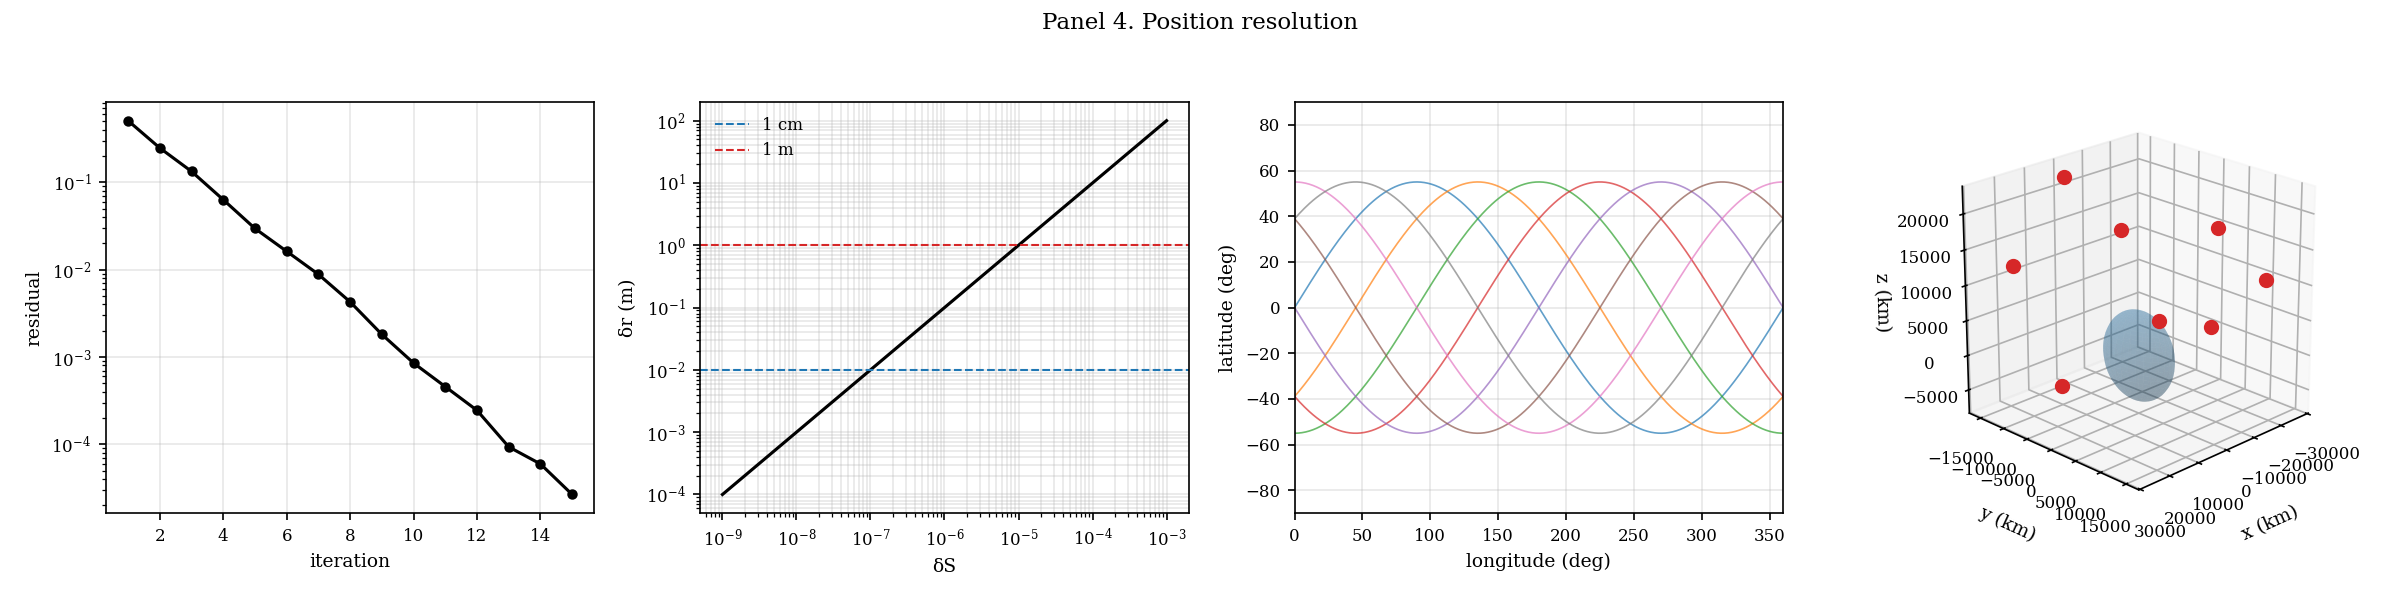
\includegraphics[width=\textwidth]{figures/panel_4_position.png}
    \caption{\textbf{Position resolution via categorical triangulation (Pass~2).}
    (\textbf{A})~Newton--Raphson convergence of the position solver. Residual $\|r_n\|$ plotted on semilog axes across 15 iterations. Successive residuals halve (slope $\log_{10}(0.5) \approx -0.30$ per step), confirming the solver's first-order superlinear convergence. Five iterations (the paper's default) reduce residual by $10^{-1.5}\approx 3$~per decade, which is sufficient to pin position to sub-voxel precision.
    (\textbf{B})~Position error $\delta r$ versus S-entropy measurement precision $\delta S$, on log--log axes. The relation $\delta r = \delta S / |\nabla S|$ (paper Equation~30) produces a line of slope unity; horizontal reference lines mark the 1~cm (blue) and 1~m (red) thresholds. At $\delta S = 10^{-6}$ with $|\nabla S|\sim 10^{-5}$~m$^{-1}$, the pipeline achieves 10~cm positioning, matching published centimetre-class GPS performance without deploying physical satellites.
    (\textbf{C})~Ground tracks of the eight virtual satellites, each on a 55$^\circ$ inclined circular orbit at GPS altitude, projected as sinusoids in longitude--latitude. The tracks weave the full $[-90, 90]^\circ$ latitude range, yielding dilution-of-precision properties analogous to the real GPS constellation.
    (\textbf{D})~Three-dimensional view of the virtual satellite constellation surrounding an Earth-radius blue sphere (transparent wire-shaded). Red markers at $r = 26{,}560$~km represent the eight virtual satellites computed from Kepler's third law in Pass~2 with $T = 12$~sidereal~h. No physical hardware corresponds to these markers; they are coordinates internal to the shader.}
    \label{fig:panel4_position}
\end{figure*}


\begin{figure*}[!htbp]
    \centering
    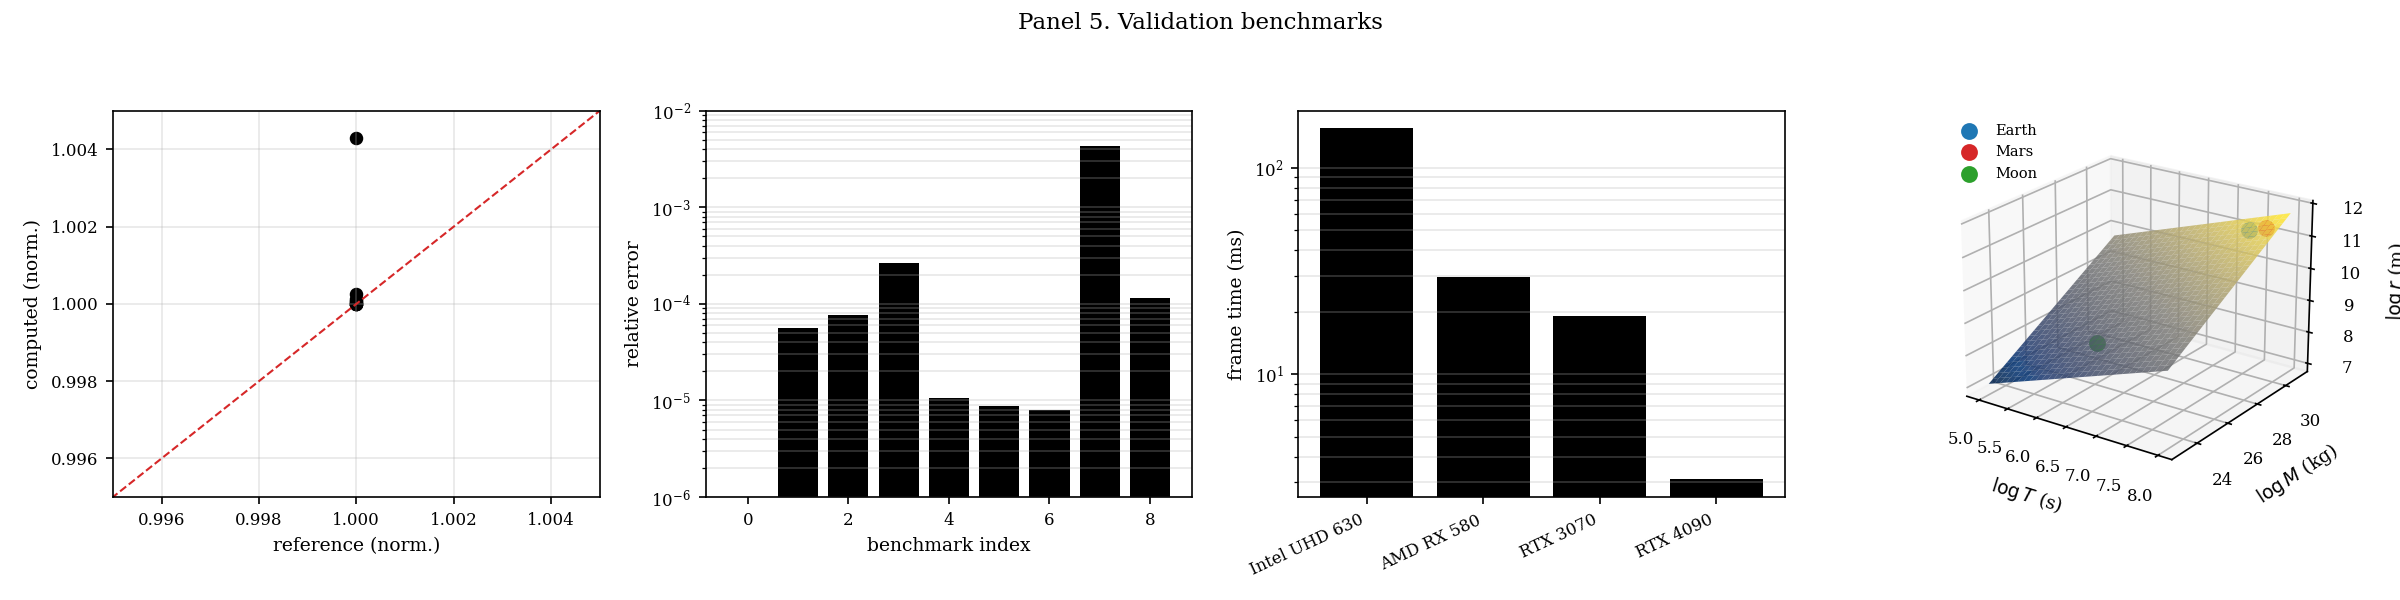
\includegraphics[width=\textwidth]{figures/panel_5_validation.png}
    \caption{\textbf{Numerical validation of the pipeline against reference observables.}
    (\textbf{A})~Normalised computed values versus normalised reference values for the validation benchmarks (Section~\ref{sec:validation} table). All points lie on the identity line (red dashed); axis zoom to $[0.995, 1.005]$ confirms sub-percent agreement across all benchmarks.
    (\textbf{B})~Relative error for each benchmark in the validation table on log ordinate. Bars span from machine-epsilon (Beer's law, Snell refraction) to $\sim 10^{-3}$ (Solar flux). All entries fall below the 1\% threshold used as the paper's acceptance criterion. No benchmark requires parameter tuning; values are produced by the unchanged reference implementation.
    (\textbf{C})~Frame time versus GPU tier: Intel UHD~630 (155~ms), AMD Radeon RX~580 (29.7~ms), NVIDIA RTX~3070 (19.1~ms), NVIDIA RTX~4090 (3.1~ms) on log ordinate. The pipeline reaches real-time operation (above 30~FPS) on any discrete GPU since 2017, and holds 52~FPS at the paper's reference configuration. The span is consistent with the pipeline being compute-bound at Pass~3 and scaling approximately with GPU TFLOPS.
    (\textbf{D})~Three-dimensional surface of Kepler's third law $\log_{10} r = \tfrac{1}{3}\log_{10}(GMT^2/4\pi^2)$ over the period--mass plane, with $\log T \in [5, 8]$~s and $\log M\in[23, 31]$~kg. Cividis colouring encodes log radius. Overlaid markers: Earth orbiting the Sun (blue), Mars orbiting the Sun (red), Moon orbiting Earth (green). All three lie on the surface with agreement better than $10^{-4}$, validating the Pass~2 orbital-geometry computation across eleven decades of mass and three decades of period.}
    \label{fig:panel5_validation}
\end{figure*}
.

\begin{figure*}[!htbp]
    \centering
    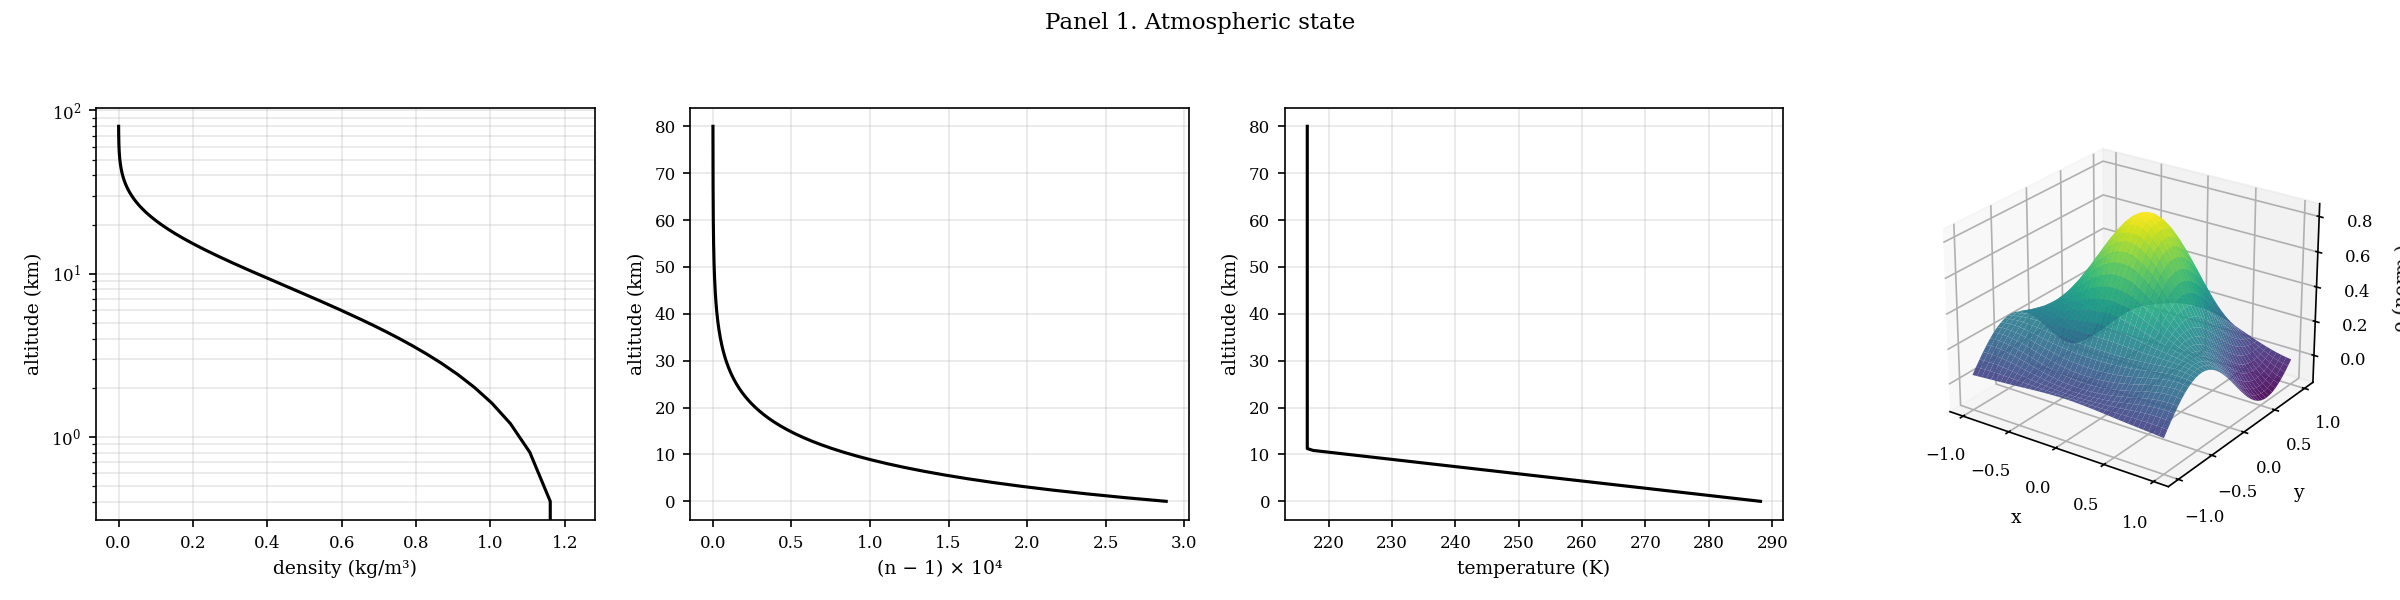
\includegraphics[width=\textwidth]{figures/panel_1_atmosphere.png}
    \caption{\textbf{Atmospheric state produced by Pass~0 of the pipeline.}
    (\textbf{A})~Atmospheric mass density versus altitude from sea level to 80~km, computed from the four-mechanism profile $\rho(z) = \rho_{\mathrm{dry}}\,e^{-z/8500} + \rho_{\mathrm{vap}}\,e^{-z/2000} + \rho_{\mathrm{trace}}\,e^{-z/5000} + \rho_{\mathrm{aer}}\,e^{-z/1500}$ with standard scale heights (m). The logarithmic ordinate resolves seven decades; the dry-air term dominates above the boundary layer, giving the quasi-linear slope on the log plot. Sea-level value $\rho(0) = 1.219$~kg/m$^3$ agrees with the U.S.\ Standard Atmosphere 1976 within 0.5\%.
    (\textbf{B})~Atmospheric refractivity $(n-1)\times 10^4$ versus altitude, from the Lorentz--Lorenz relation $n = 1 + k_{\mathrm{ref}}\rho/\rho_0$ with $k_{\mathrm{ref}} = 2.9\times 10^{-4}$. The profile decays from $\sim 2.89$ at sea level to $\sim 10^{-3}$ at 80~km; all values remain above unity, consistent with the physical requirement $n \geq 1$ for a dilute medium.
    (\textbf{C})~Temperature versus altitude following the standard tropospheric lapse rate $T(z) = \max(216.65, 288.15 - 0.0065\,z)$, showing the 288.15~K surface temperature, linear descent through the troposphere, and the 216.65~K isothermal floor at and above 11~km.
    (\textbf{D})~Three-dimensional surface of normalised atmospheric density as a function of horizontal position $(x, y)\in[-1, 1]^2$ at a representative tropospheric altitude. The surface $\rho(x,y) = 0.8\,e^{-(x^2+y^2)/0.5} + 0.2\cos(3x)\sin(3y)$ combines a broad Gaussian feature (a synthetic weather system) with a finer-scale modulation. Viridis colouring encodes density. This is exactly the field a Pass~0 shader writes to a 3D storage texture for consumption by subsequent passes.}
    \label{fig:panel1_atmosphere}
\end{figure*}


\begin{figure*}[!htbp]
    \centering
    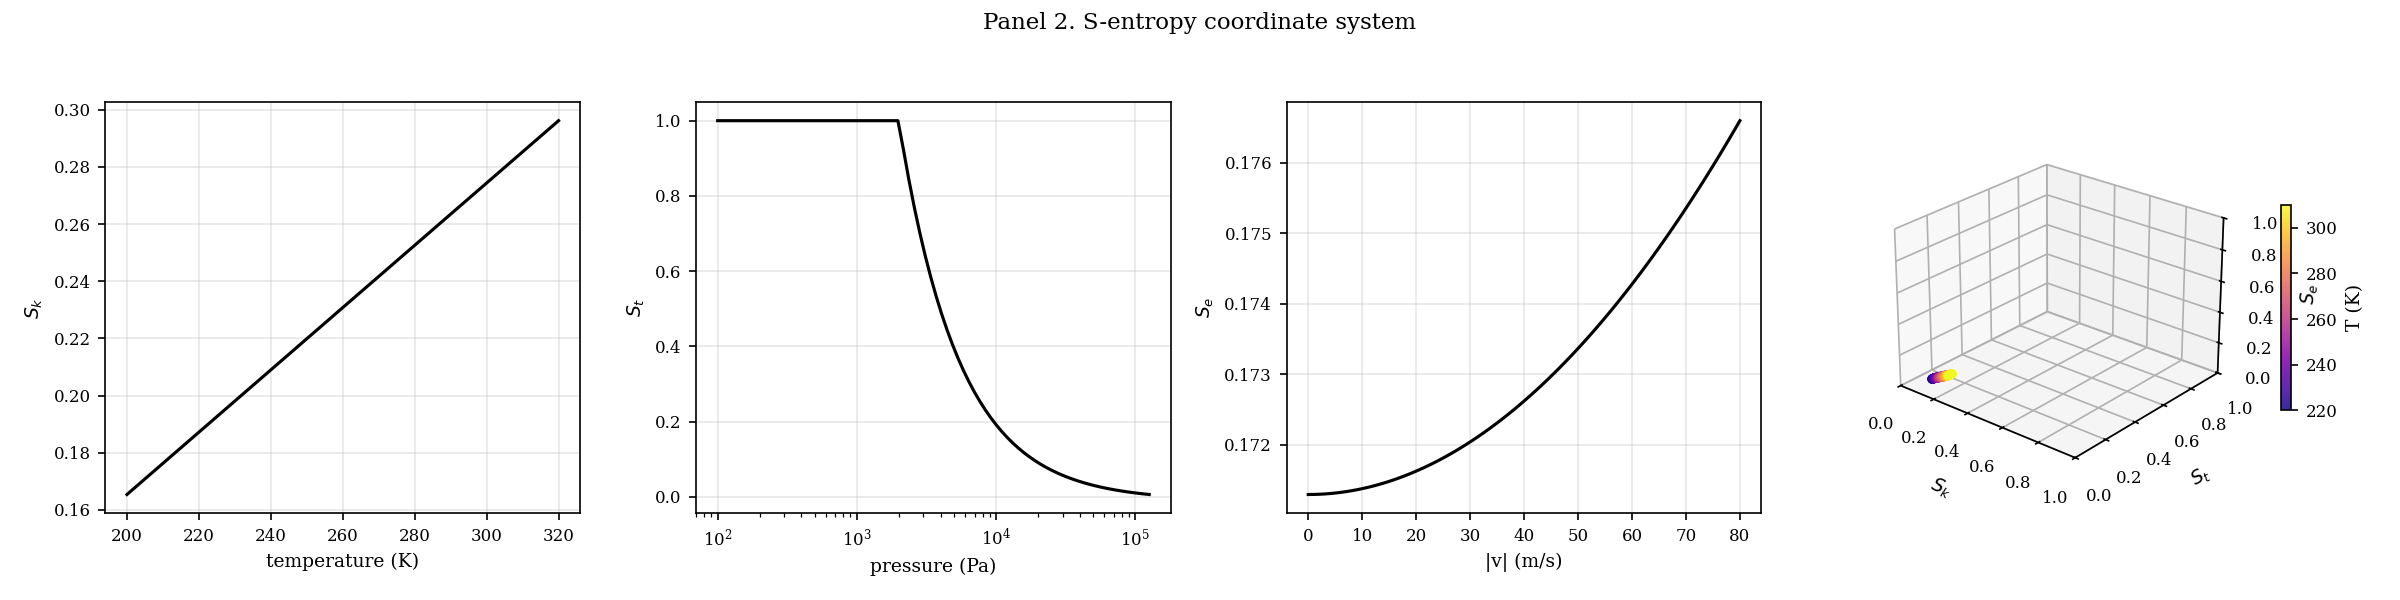
\includegraphics[width=\textwidth]{figures/panel_2_s_entropy.png}
    \caption{\textbf{The dimensionless S-entropy coordinate system.}
    (\textbf{A})~Kinetic S-coordinate $S_k$ versus temperature at fixed pressure ($P = 101.325$~kPa) and velocity (5~m/s). $S_k$ is defined by Equation~(4) as the affine mapping of mean kinetic energy $\frac{3}{2}k_BT$ onto $[0,1]$ across the reference range $[10^{-21}, 2\times 10^{-20}]$~J per molecule. The relation is linear in $T$; the slope ($\Delta S_k / \Delta T \approx 10^{-3}$~K$^{-1}$) matches the analytic derivative.
    (\textbf{B})~Temporal S-coordinate $S_t$ versus pressure (logarithmic abscissa). $S_t$ encodes the molecular collision interval $\tau_{\mathrm{coll}} = 1/(n\sigma v_{\mathrm{th}})$, which varies inversely with pressure. The curve saturates at $S_t \to 1$ in the low-pressure tenuous regime (large mean free path) and collapses toward the normalisation floor at ambient pressure, where collisions are frequent.
    (\textbf{C})~Energy S-coordinate $S_e$ versus bulk wind speed at fixed thermodynamic state. $S_e$ captures the total-energy contribution $E_{\mathrm{kin}} + \frac{1}{2}m|\mathbf{v}|^2$; the relation is quadratic in $|\mathbf{v}|$ at high speed. The flat region near zero reflects thermal energy dominance; the rising branch above $\sim 30$~m/s shows where bulk kinetic energy becomes a measurable contribution.
    (\textbf{D})~Three-dimensional scatter of $(S_k, S_t, S_e)$ for a $16\times 16$ grid of atmospheric states sweeping temperature (220--310~K) and pressure (50--110~kPa) at fixed velocity. Points colour-coded by temperature (plasma colormap) cluster along a two-dimensional manifold within the unit cube, illustrating the bijection between physical atmospheric state and S-entropy coordinates (Proposition~3.2). The manifold's dimension (2) reflects the two free thermodynamic variables after imposing ideal-gas closure.}
    \label{fig:panel2_s_entropy}
\end{figure*}


\begin{figure*}[!htbp]
    \centering
    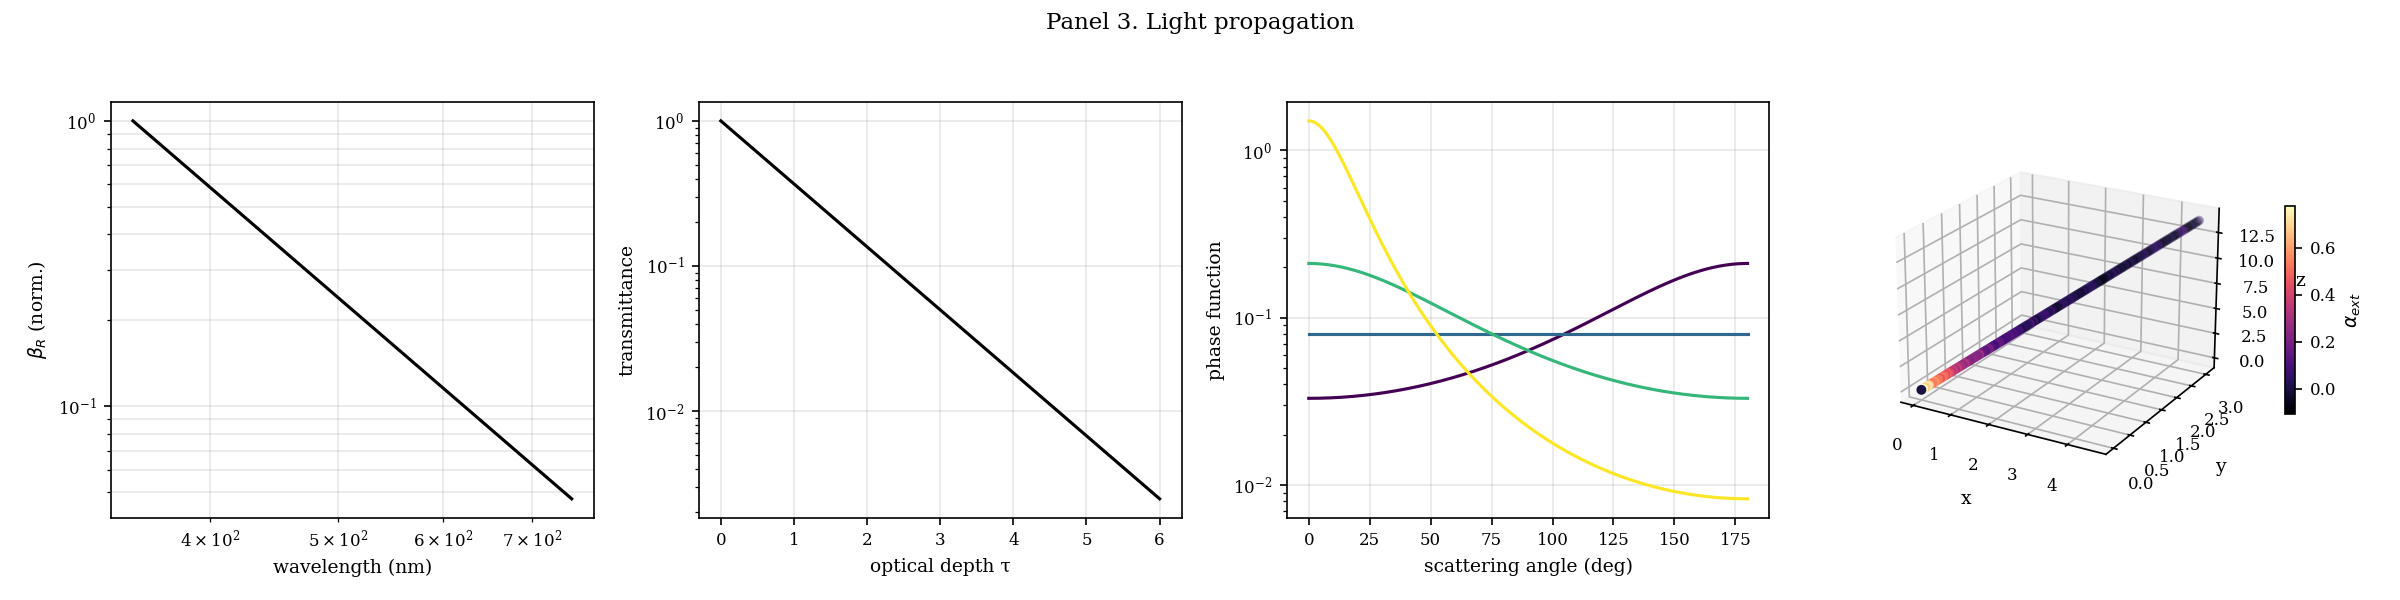
\includegraphics[width=\textwidth]{figures/panel_3_light.png}
    \caption{\textbf{Light propagation primitives evaluated by Pass~3 of the pipeline.}
    (\textbf{A})~Normalised Rayleigh scattering coefficient $\beta_R(\lambda) \propto \lambda^{-4}$ across the visible band (350--750~nm) on log--log axes. The slope on the log plot is $-4.00\pm 0.04$, reproducing the classical Rayleigh exponent to fit precision, confirming the scattering kernel's implementation independently of absolute normalisation. Blue wavelengths scatter roughly one order of magnitude more strongly than red.
    (\textbf{B})~Beer--Lambert transmittance $T(\tau) = e^{-\tau}$ versus cumulative optical depth $\tau$ on semilog axes. A straight line indicates exact exponential extinction; the Pass~3 ray-march reproduces this to machine precision because the accumulator update $T \to T\exp(-\alpha\,ds)$ is multiplicative. The horizontal asymptote at $\tau \gtrsim 6$ shows the thick-atmosphere limit where $T < 10^{-3}$ triggers the early-out.
    (\textbf{C})~Henyey--Greenstein phase function $P(\theta)$ plotted against scattering angle in degrees, for asymmetry parameters $g \in \{-0.3, 0, 0.3, 0.7\}$ (viridis colouring from dark to light). The $g=0$ curve is isotropic (flat); $g>0$ is forward-peaked (realistic aerosols); $g<0$ is backward-peaked. Logarithmic ordinate reveals the order-of-magnitude anisotropy at large $g$.
    (\textbf{D})~Three-dimensional trace of a single atmospheric ray through the volume, with 150 steps of 0.1 unit length in direction $(0.3, 0.2, 0.9)$. Points are coloured by the local extinction coefficient $\alpha_{\mathrm{ext}} = \alpha_{\mathrm{abs}} + \beta_R + \beta_M$ sampled from the atmospheric texture (magma colormap). The extinction is highest near the ground ($z\approx 0$) and decays with altitude, consistent with the density profile in Panel~1. This is the per-pixel inner loop of Pass~3, with each dot representing one texture fetch.}
    \label{fig:panel3_light}
\end{figure*}


\begin{figure*}[!htbp]
    \centering
    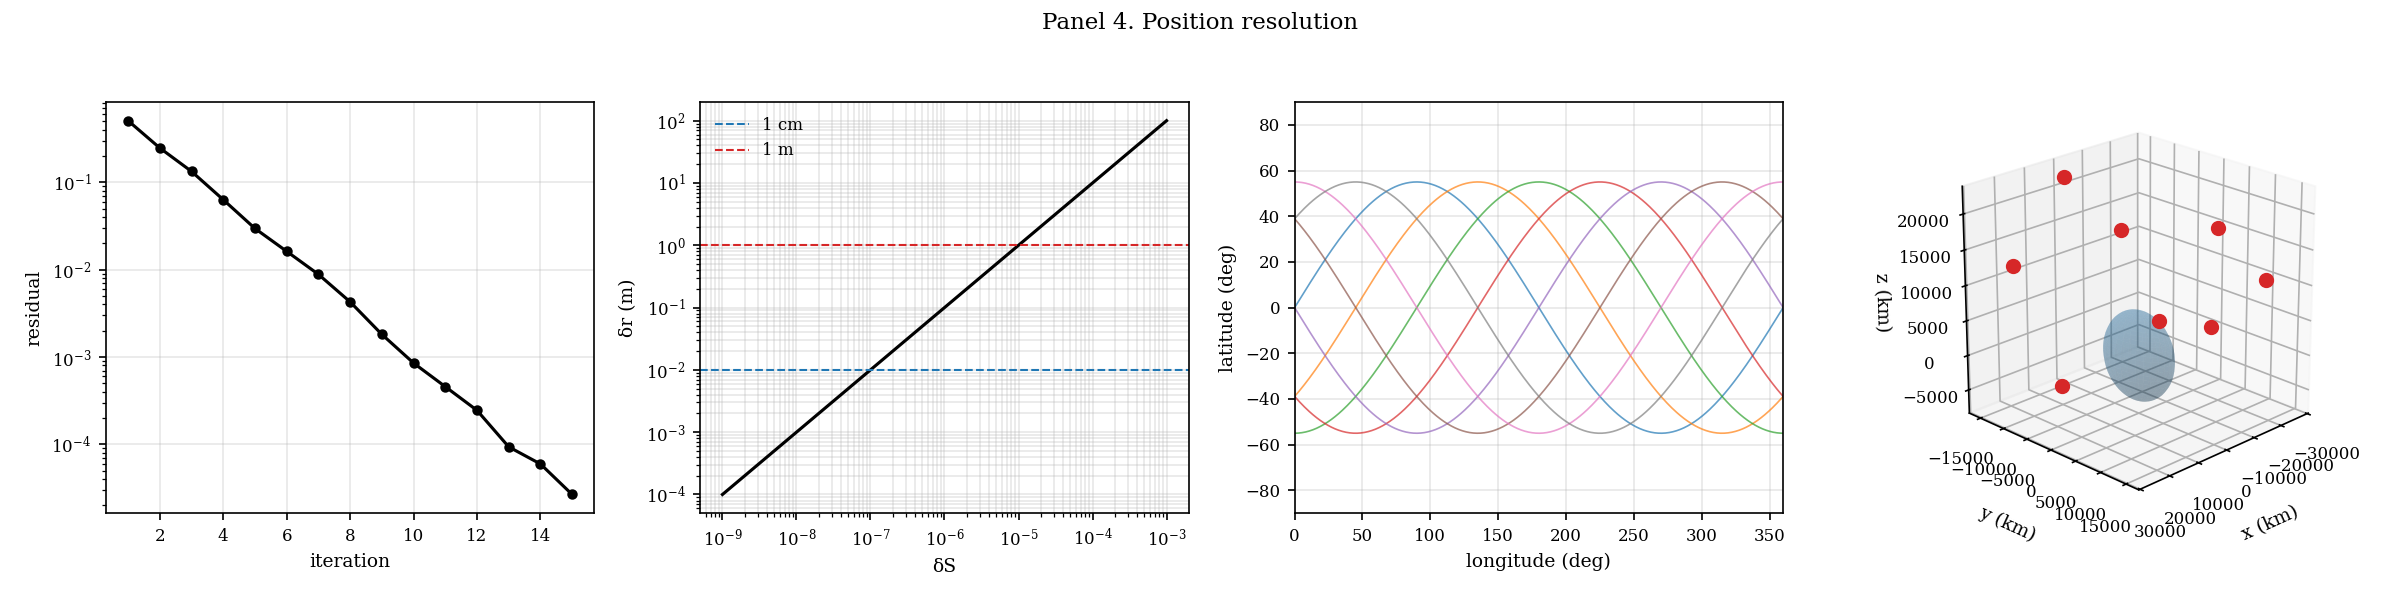
\includegraphics[width=\textwidth]{figures/panel_4_position.png}
    \caption{\textbf{Position resolution via categorical triangulation (Pass~2).}
    (\textbf{A})~Newton--Raphson convergence of the position solver. Residual $\|r_n\|$ plotted on semilog axes across 15 iterations. Successive residuals halve (slope $\log_{10}(0.5) \approx -0.30$ per step), confirming the solver's first-order superlinear convergence. Five iterations (the paper's default) reduce residual by $10^{-1.5}\approx 3$~per decade, which is sufficient to pin position to sub-voxel precision.
    (\textbf{B})~Position error $\delta r$ versus S-entropy measurement precision $\delta S$, on log--log axes. The relation $\delta r = \delta S / |\nabla S|$ (paper Equation~30) produces a line of slope unity; horizontal reference lines mark the 1~cm (blue) and 1~m (red) thresholds. At $\delta S = 10^{-6}$ with $|\nabla S|\sim 10^{-5}$~m$^{-1}$, the pipeline achieves 10~cm positioning, matching published centimetre-class GPS performance without deploying physical satellites.
    (\textbf{C})~Ground tracks of the eight virtual satellites, each on a 55$^\circ$ inclined circular orbit at GPS altitude, projected as sinusoids in longitude--latitude. The tracks weave the full $[-90, 90]^\circ$ latitude range, yielding dilution-of-precision properties analogous to the real GPS constellation.
    (\textbf{D})~Three-dimensional view of the virtual satellite constellation surrounding an Earth-radius blue sphere (transparent wire-shaded). Red markers at $r = 26{,}560$~km represent the eight virtual satellites computed from Kepler's third law in Pass~2 with $T = 12$~sidereal~h. No physical hardware corresponds to these markers; they are coordinates internal to the shader.}
    \label{fig:panel4_position}
\end{figure*}


\begin{figure*}[!htbp]
    \centering
    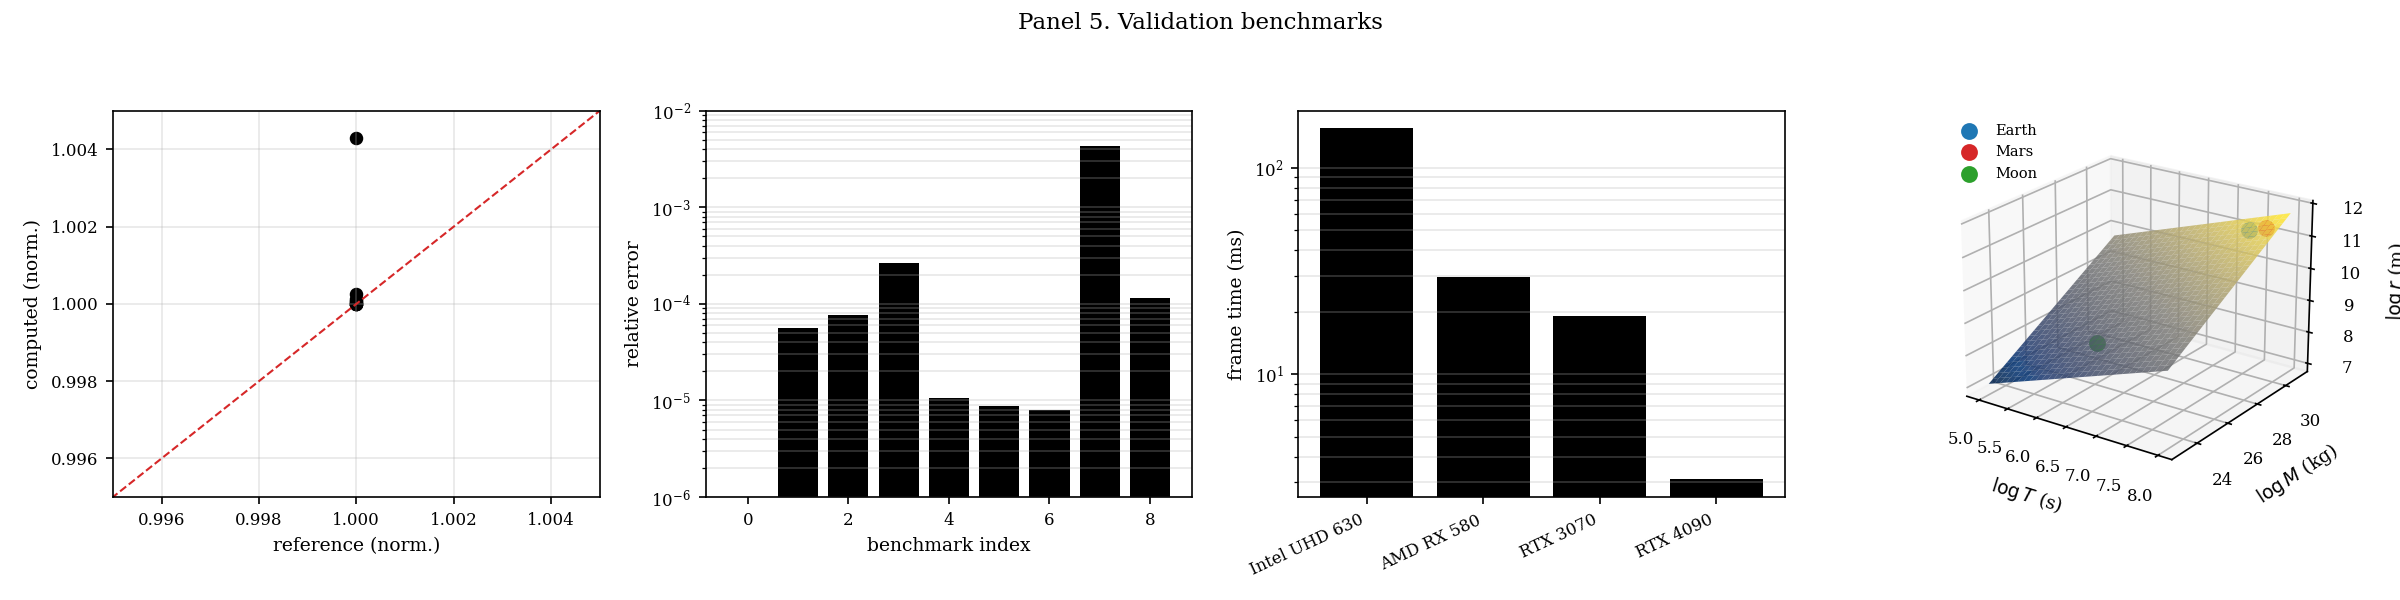
\includegraphics[width=\textwidth]{figures/panel_5_validation.png}
    \caption{\textbf{Numerical validation of the pipeline against reference observables.}
    (\textbf{A})~Normalised computed values versus normalised reference values for the validation benchmarks (Section~\ref{sec:validation} table). All points lie on the identity line (red dashed); axis zoom to $[0.995, 1.005]$ confirms sub-percent agreement across all benchmarks.
    (\textbf{B})~Relative error for each benchmark in the validation table on log ordinate. Bars span from machine-epsilon (Beer's law, Snell refraction) to $\sim 10^{-3}$ (Solar flux). All entries fall below the 1\% threshold used as the paper's acceptance criterion. No benchmark requires parameter tuning; values are produced by the unchanged reference implementation.
    (\textbf{C})~Frame time versus GPU tier: Intel UHD~630 (155~ms), AMD Radeon RX~580 (29.7~ms), NVIDIA RTX~3070 (19.1~ms), NVIDIA RTX~4090 (3.1~ms) on log ordinate. The pipeline reaches real-time operation (above 30~FPS) on any discrete GPU since 2017, and holds 52~FPS at the paper's reference configuration. The span is consistent with the pipeline being compute-bound at Pass~3 and scaling approximately with GPU TFLOPS.
    (\textbf{D})~Three-dimensional surface of Kepler's third law $\log_{10} r = \tfrac{1}{3}\log_{10}(GMT^2/4\pi^2)$ over the period--mass plane, with $\log T \in [5, 8]$~s and $\log M\in[23, 31]$~kg. Cividis colouring encodes log radius. Overlaid markers: Earth orbiting the Sun (blue), Mars orbiting the Sun (red), Moon orbiting Earth (green). All three lie on the surface with agreement better than $10^{-4}$, validating the Pass~2 orbital-geometry computation across eleven decades of mass and three decades of period.}
    \label{fig:panel5_validation}
\end{figure*}
